\pdfoutput=1
\documentclass[twoside,11pt]{article}
\usepackage{amsmath,amssymb,amsthm,mathtools}
\usepackage[preprint]{jmlr2e}
\usepackage{booktabs}
\usepackage{xurl}
\usepackage{adjustbox}
\usepackage[dvipsnames,table]{xcolor}
\usepackage{microtype}
\usepackage{subcaption}
\captionsetup{format=hang,font=normalsize,labelfont=normalfont,textfont=normalfont}
\renewcommand{\qedsymbol}{\ensuremath{\blacksquare}}
% Reference numbers in Online Appendix 1 are fixed to the accompanying supplement.
\makeatletter
\@namedef{r@supp:stages}{{S1}{1}{}{section.1}{https://github.com/yspennstate/neural-means-kernel-corrections/raw/refs/heads/main/paper/supplement.pdf}}
\@namedef{r@sec:theory-sym}{{S1.1}{1}{}{subsection.1.1}{https://github.com/yspennstate/neural-means-kernel-corrections/raw/refs/heads/main/paper/supplement.pdf}}
\@namedef{r@prop:sym}{{S1.1}{1}{symmetrization}{theorem.1.1}{https://github.com/yspennstate/neural-means-kernel-corrections/raw/refs/heads/main/paper/supplement.pdf}}
\@namedef{r@eq:refiner-defect}{{S1.1}{2}{}{equation.1.1}{https://github.com/yspennstate/neural-means-kernel-corrections/raw/refs/heads/main/paper/supplement.pdf}}
\@namedef{r@sec:theory-kf}{{S1.2}{2}{}{subsection.1.2}{https://github.com/yspennstate/neural-means-kernel-corrections/raw/refs/heads/main/paper/supplement.pdf}}
\@namedef{r@eq:kf}{{S1.2}{3}{}{equation.1.2}{https://github.com/yspennstate/neural-means-kernel-corrections/raw/refs/heads/main/paper/supplement.pdf}}
\@namedef{r@prop:kf}{{S1.2}{3}{KF loss is a leave-half-out estimate}{theorem.1.2}{https://github.com/yspennstate/neural-means-kernel-corrections/raw/refs/heads/main/paper/supplement.pdf}}
\@namedef{r@sec:theory-stack}{{S1.3}{3}{}{subsection.1.3}{https://github.com/yspennstate/neural-means-kernel-corrections/raw/refs/heads/main/paper/supplement.pdf}}
\@namedef{r@prop:stack}{{S1.3}{3}{validation stacking}{theorem.1.3}{https://github.com/yspennstate/neural-means-kernel-corrections/raw/refs/heads/main/paper/supplement.pdf}}
\@namedef{r@lem:select}{{S1.4}{4}{validated selection}{theorem.1.4}{https://github.com/yspennstate/neural-means-kernel-corrections/raw/refs/heads/main/paper/supplement.pdf}}
\@namedef{r@prop:affine}{{S1.5}{4}{per-pixel affine stacking}{theorem.1.5}{https://github.com/yspennstate/neural-means-kernel-corrections/raw/refs/heads/main/paper/supplement.pdf}}
\@namedef{r@cor:certificate}{{S1.6}{5}{capacity bound for a fixed composite correction class}{theorem.1.6}{https://github.com/yspennstate/neural-means-kernel-corrections/raw/refs/heads/main/paper/supplement.pdf}}
\@namedef{r@lem:kappa}{{S1.7}{6}{uniform bound on kernel ridge weights}{theorem.1.7}{https://github.com/yspennstate/neural-means-kernel-corrections/raw/refs/heads/main/paper/supplement.pdf}}
\@namedef{r@supp:rules}{{S2}{6}{}{section.2}{https://github.com/yspennstate/neural-means-kernel-corrections/raw/refs/heads/main/paper/supplement.pdf}}
\@namedef{r@prop:margin}{{S2.1}{6}{margin law for a threshold rule}{theorem.2.1}{https://github.com/yspennstate/neural-means-kernel-corrections/raw/refs/heads/main/paper/supplement.pdf}}
\@namedef{r@proof:prop:margin}{{S2}{7}{}{theorem.2.1}{https://github.com/yspennstate/neural-means-kernel-corrections/raw/refs/heads/main/paper/supplement.pdf}}
\@namedef{r@prop:percoord}{{S2.2}{7}{per-coordinate combination under diagonal metrics}{theorem.2.2}{https://github.com/yspennstate/neural-means-kernel-corrections/raw/refs/heads/main/paper/supplement.pdf}}
\@namedef{r@cor:percoordw}{{S2.3}{8}{weighted metrics and the reported error}{theorem.2.3}{https://github.com/yspennstate/neural-means-kernel-corrections/raw/refs/heads/main/paper/supplement.pdf}}
\@namedef{r@prop:selectcoord}{{S2.4}{8}{empirical per-coordinate selection}{theorem.2.4}{https://github.com/yspennstate/neural-means-kernel-corrections/raw/refs/heads/main/paper/supplement.pdf}}
\@namedef{r@prop:aniso}{{S2.5}{9}{finite-design rank truncation}{theorem.2.5}{https://github.com/yspennstate/neural-means-kernel-corrections/raw/refs/heads/main/paper/supplement.pdf}}
\@namedef{r@supp:conf}{{S3}{9}{}{section.3}{https://github.com/yspennstate/neural-means-kernel-corrections/raw/refs/heads/main/paper/supplement.pdf}}
\@namedef{r@eq:conf}{{S3.1}{9}{}{equation.3.1}{https://github.com/yspennstate/neural-means-kernel-corrections/raw/refs/heads/main/paper/supplement.pdf}}
\@namedef{r@prop:conf}{{S3.1}{10}{finite-sample coverage}{theorem.3.1}{https://github.com/yspennstate/neural-means-kernel-corrections/raw/refs/heads/main/paper/supplement.pdf}}
\@namedef{r@rem:covlaw}{{S3.2}{10}{conditional reference law for realized coverage}{theorem.3.2}{https://github.com/yspennstate/neural-means-kernel-corrections/raw/refs/heads/main/paper/supplement.pdf}}
\@namedef{r@supp:benchmark}{{S4}{10}{}{section.4}{https://github.com/yspennstate/neural-means-kernel-corrections/raw/refs/heads/main/paper/supplement.pdf}}
\@namedef{r@sec:suite}{{S4.1}{10}{}{subsection.4.1}{https://github.com/yspennstate/neural-means-kernel-corrections/raw/refs/heads/main/paper/supplement.pdf}}
\@namedef{r@tab:suite}{{S4.1}{11}{Additional benchmark survey. Published reference mean relative $L^2$ test error on each problem (per-problem methods tuned by their authors), compared with the common training protocol on training splits and grids that differ from the baselines' in the cases noted in the text: single runs, except the two rows marked three seeds (mean $\pm $ standard deviation, exact solve on 19{,}000 pairs, output rank 400)}{table.caption.1}{https://github.com/yspennstate/neural-means-kernel-corrections/raw/refs/heads/main/paper/supplement.pdf}}
\@namedef{r@sec:symcheck}{{S4.2}{11}{}{subsection.4.2}{https://github.com/yspennstate/neural-means-kernel-corrections/raw/refs/heads/main/paper/supplement.pdf}}
\@namedef{r@supp:deff}{{S5}{12}{}{section.5}{https://github.com/yspennstate/neural-means-kernel-corrections/raw/refs/heads/main/paper/supplement.pdf}}
\@namedef{r@sec:theory-rmt}{{S5.1}{12}{}{subsection.5.1}{https://github.com/yspennstate/neural-means-kernel-corrections/raw/refs/heads/main/paper/supplement.pdf}}
\@namedef{r@lem:deff}{{S5.1}{12}{effective dimension and the empirical Stieltjes transform}{theorem.5.1}{https://github.com/yspennstate/neural-means-kernel-corrections/raw/refs/heads/main/paper/supplement.pdf}}
\@namedef{r@cor:mp}{{S5.2}{12}{effective dimension under a Mar\v {c}enko--Pastur limit}{theorem.5.2}{https://github.com/yspennstate/neural-means-kernel-corrections/raw/refs/heads/main/paper/supplement.pdf}}
\@namedef{r@supp:experiments}{{S6}{13}{}{section.6}{https://github.com/yspennstate/neural-means-kernel-corrections/raw/refs/heads/main/paper/supplement.pdf}}
\@namedef{r@sec:ablation}{{S6.1}{13}{}{subsection.6.1}{https://github.com/yspennstate/neural-means-kernel-corrections/raw/refs/heads/main/paper/supplement.pdf}}
\@namedef{r@sec:errors}{{S6.2}{13}{}{subsection.6.2}{https://github.com/yspennstate/neural-means-kernel-corrections/raw/refs/heads/main/paper/supplement.pdf}}
\@namedef{r@tab:ablation}{{S6.1}{14}{Component contributions in the high-data pipeline. Mean relative $L^2$ test error under the 20000-sample protocol; ``+'' rows are cumulative. All rows are mean $\pm $ standard deviation over ten seeds; the last two are the second experiment of Section~\ref {sec:seeds}}{table.caption.2}{https://github.com/yspennstate/neural-means-kernel-corrections/raw/refs/heads/main/paper/supplement.pdf}}
\@namedef{r@fig:corr}{{S6.1}{14}{Centered correlation of per-sample normalized residuals on the validation split, six members, averaged over the ten seeds of the second experiment. Across seeds and pairs the entries range between $0.82$ and $0.98$. The mean over pairs is $0.919\pm 0.005$ across seeds; the kernel predictor has correlation \corrKerLo --\corrKerHi {} with the normalized-MSE network at every seed. These centered correlations differ from the uncentered alignments summarized in Section~\ref {sec:diversity}}{figure.caption.3}{https://github.com/yspennstate/neural-means-kernel-corrections/raw/refs/heads/main/paper/supplement.pdf}}
\@namedef{r@fig:shared}{{S6.2}{15}{Spatial and spectral structure of the shared residual $c$ (across-member mean of the residual fields), at one seed. Left to right: rms of $c$ over the grid; rms of the member-specific remainders; radial DCT band energies of the stress fields, of $c$, and of the member-specific remainders; and the norm of $c$ against the output norm, whose correlation is $0.01$}{figure.caption.4}{https://github.com/yspennstate/neural-means-kernel-corrections/raw/refs/heads/main/paper/supplement.pdf}}
\@namedef{r@sec:spectra}{{S6.3}{15}{}{subsection.6.3}{https://github.com/yspennstate/neural-means-kernel-corrections/raw/refs/heads/main/paper/supplement.pdf}}
\@namedef{r@sec:cost}{{S6.4}{15}{}{subsection.6.4}{https://github.com/yspennstate/neural-means-kernel-corrections/raw/refs/heads/main/paper/supplement.pdf}}
\@namedef{r@tab:norms}{{S6.2}{17}{Fitted-norm diagnostic of the residual correction at seed $0$ of the complete-schedule experiment: the same validated correction kernel (scale multiplier $2$, nugget $10^{-3}$, median length scale) ridge-fitted to the raw stress fields and to the six-member stack residuals on the training split. $\|\widehat r\|_K^2=\operatorname {tr}(\alpha ^\top K\alpha )$ is the squared RKHS norm of the fitted function; the last column divides it by the energy of the fitted label array. The residual labels mix foldwise kernel predictions and in-sample neural predictions, so these numbers are not identified as lower bounds for the native-space norm of the deployed residual. The ratios depend on the selected nugget and scale. Much of the raw ratio reflects output amplitude: per unit energy the residual's fitted norm is \normRatioNorm {} times smaller at this seed, not \normRatio {}; at seeds $1$ and $2$, whose corrections chose scale multipliers $1$ and $2$, the raw ratios are \normRatioLo {} and $4300$ and the normalized ones \normRatioNormLo {} and $7.6$}{table.caption.5}{https://github.com/yspennstate/neural-means-kernel-corrections/raw/refs/heads/main/paper/supplement.pdf}}
\@namedef{r@fig:uq}{{S6.3}{17}{Uncertainty measures for the six-member correction at seed 0. Calibration uses $1000$ test-block cases and evaluation uses the other $19000$, as in Section~\ref {sec:uq}. Left: the Gaussian process posterior standard deviation $P_\lambda $ against relative error; the association is negative (Pearson $-0.33$) because large-amplitude outputs have small relative error. Middle: decile calibration of $P_\lambda $ against absolute error $\|e(u)\|_2$; the association is weak (Pearson $0.05$). Right: coverage of the $P_\lambda $-scaled $90\%$ band within each decile of $P_\lambda $: $91.4\%$ overall, but from $69\%$ in the lowest decile to $99.9\%$ in the highest, so coverage varies strongly with the design factor despite an overall value close to the nominal level. Across the ten seeds the same band has coverage $\uqPlamSix \pm \uqPlamSixSd \%$ at the nominal \uqCoverNom \% level, inside the i.i.d.-continuous Beta--binomial reference interval at ten seeds of ten; the constant-radius band is the narrower of the two (Section~\ref {sec:uq})}{figure.caption.6}{https://github.com/yspennstate/neural-means-kernel-corrections/raw/refs/heads/main/paper/supplement.pdf}}
\@namedef{r@fig:scaling}{{S6.4}{18}{Structural-mechanics learning curves. The first $N+1000$ rows of the training pool are used, with the final $1000$ reserved for validation and the first $N$ for fitting. The validation split is fixed across seeds at each $N$ and changes with $N$; evaluation uses the full test block. The curves give mean relative test error for the normalized-MSE network (mean and standard deviation over ten seeds) and deterministic Mat\'ern kernel ridge on loads, with both axes logarithmic. The horizontal lines mark the six-member pipeline at $19000$ samples and the quoted PARA-Net result. Error bars are smaller than the markers above $4000$}{figure.caption.7}{https://github.com/yspennstate/neural-means-kernel-corrections/raw/refs/heads/main/paper/supplement.pdf}}
\@namedef{r@fig:seedspread}{{S6.5}{21}{Left: the corrected pipeline's test error at each of the ten seeds (points), their mean (dashed), and the five published benchmark errors on the same axis (grey). These show the variability of our pipeline; comparable seed distributions are unavailable for the published methods. Right: test error at successive pipeline stages for each seed, with the stage means marked. Fitting per-pixel weights lowers the mean; seed spreads at each stage are reported in the text}{figure.caption.8}{https://github.com/yspennstate/neural-means-kernel-corrections/raw/refs/heads/main/paper/supplement.pdf}}
\@namedef{r@supp:oco2}{{S7}{21}{}{section.7}{https://github.com/yspennstate/neural-means-kernel-corrections/raw/refs/heads/main/paper/supplement.pdf}}
\@namedef{r@tab:aniso}{{S7.1}{22}{The raw-input kernel refit at nested training sizes, ten seeds per band. ``Rank'' counts singular values of the fitting-set matrix $B=X_{\rm tr}^{\dagger }Z$ holding $99\%$ of the squared energy, out of the input dimension. The exponent difference is paired within seed; its standard deviation is over seeds. The last column is the isotropic-to-adapted error ratio at $n=18000$. The slopes are descriptive fits over the finite sizes tested}{table.caption.9}{https://github.com/yspennstate/neural-means-kernel-corrections/raw/refs/heads/main/paper/supplement.pdf}}
\@namedef{r@fig:floor}{{S7.1}{23}{Exploratory WCO2 Fourier-feature sweep. The legend identifies bandwidths; the dashed line is the SiLU error of $16.37\%$. Three bandwidths nearly coincide in the upper left. Errors and correlations are rounded summaries of the exploratory measurements. The admission calculations in Section~\ref {sec:secmom-margin} use exact uncentered second moments}{figure.caption.10}{https://github.com/yspennstate/neural-means-kernel-corrections/raw/refs/heads/main/paper/supplement.pdf}}
\@namedef{r@sec:scaling}{{S7.2}{24}{}{subsection.7.2}{https://github.com/yspennstate/neural-means-kernel-corrections/raw/refs/heads/main/paper/supplement.pdf}}
\@namedef{r@fig:ocoscaling}{{S7.2}{25}{Error against training-set size. Left: the OCO-2 O2 task, reduced error of the corrected surrogate at one seed, from the data-scaling run; a finite-range log--log fit has slope $-0.68$, and the error is $4.3\%$ at $n=17700$, against the $4.12\%$ the ten-seed pipeline reaches on all $18000$ pairs (dotted). Right: ClimSim, test $R^2$ over the active outputs defined in the text, at one, two and three and a half million training samples --- five seeds at one million and three at each of the larger sizes, error bars over seeds. No crossover between the two families is observed over this range. Each kernel is fitted on $6000$ rows, so its nearly constant error across nominal training sizes reflects that fixed fitting budget. The separate kernel-budget comparison is reported in the text. The neural mean has higher $R^2$; the published baseline (dotted) is shown for orientation; the protocols are not matched}{figure.caption.11}{https://github.com/yspennstate/neural-means-kernel-corrections/raw/refs/heads/main/paper/supplement.pdf}}
\@namedef{r@app:proofs}{{S8}{25}{}{section.8}{https://github.com/yspennstate/neural-means-kernel-corrections/raw/refs/heads/main/paper/supplement.pdf}}
\@namedef{r@proof:prop:sym}{{S8.1}{25}{}{subsection.8.1}{https://github.com/yspennstate/neural-means-kernel-corrections/raw/refs/heads/main/paper/supplement.pdf}}
\@namedef{r@proof:prop:kf}{{S8.2}{26}{}{subsection.8.2}{https://github.com/yspennstate/neural-means-kernel-corrections/raw/refs/heads/main/paper/supplement.pdf}}
\@namedef{r@proof:prop:stack}{{S8.3}{26}{}{subsection.8.3}{https://github.com/yspennstate/neural-means-kernel-corrections/raw/refs/heads/main/paper/supplement.pdf}}
\@namedef{r@proof:lem:select}{{S8.4}{27}{}{subsection.8.4}{https://github.com/yspennstate/neural-means-kernel-corrections/raw/refs/heads/main/paper/supplement.pdf}}
\@namedef{r@proof:prop:affine}{{S8.5}{27}{}{subsection.8.5}{https://github.com/yspennstate/neural-means-kernel-corrections/raw/refs/heads/main/paper/supplement.pdf}}
\@namedef{r@proof:cor:floorpinch}{{S8.6}{28}{}{subsection.8.6}{https://github.com/yspennstate/neural-means-kernel-corrections/raw/refs/heads/main/paper/supplement.pdf}}
\@namedef{r@proof:cor:certificate}{{S8.7}{28}{}{subsection.8.7}{https://github.com/yspennstate/neural-means-kernel-corrections/raw/refs/heads/main/paper/supplement.pdf}}
\@namedef{r@proof:lem:kappa}{{S8.8}{29}{}{subsection.8.8}{https://github.com/yspennstate/neural-means-kernel-corrections/raw/refs/heads/main/paper/supplement.pdf}}
\@namedef{r@proof:cor:signed}{{S8.9}{29}{}{subsection.8.9}{https://github.com/yspennstate/neural-means-kernel-corrections/raw/refs/heads/main/paper/supplement.pdf}}
\@namedef{r@proof:prop:secmom}{{S8.10}{30}{}{subsection.8.10}{https://github.com/yspennstate/neural-means-kernel-corrections/raw/refs/heads/main/paper/supplement.pdf}}
\@namedef{r@proof:cor:floor}{{S8.11}{30}{}{subsection.8.11}{https://github.com/yspennstate/neural-means-kernel-corrections/raw/refs/heads/main/paper/supplement.pdf}}
\@namedef{r@proof:thm:blockfloor}{{S8.12}{30}{}{subsection.8.12}{https://github.com/yspennstate/neural-means-kernel-corrections/raw/refs/heads/main/paper/supplement.pdf}}
\@namedef{r@proof:prop:exchange}{{S8.13}{31}{}{subsection.8.13}{https://github.com/yspennstate/neural-means-kernel-corrections/raw/refs/heads/main/paper/supplement.pdf}}
\@namedef{r@proof:prop:percoord}{{S8.14}{31}{}{subsection.8.14}{https://github.com/yspennstate/neural-means-kernel-corrections/raw/refs/heads/main/paper/supplement.pdf}}
\@namedef{r@proof:cor:percoordw}{{S8.15}{31}{}{subsection.8.15}{https://github.com/yspennstate/neural-means-kernel-corrections/raw/refs/heads/main/paper/supplement.pdf}}
\@namedef{r@proof:prop:selectcoord}{{S8.16}{32}{}{subsection.8.16}{https://github.com/yspennstate/neural-means-kernel-corrections/raw/refs/heads/main/paper/supplement.pdf}}
\@namedef{r@proof:prop:pullback}{{S8.17}{32}{}{subsection.8.17}{https://github.com/yspennstate/neural-means-kernel-corrections/raw/refs/heads/main/paper/supplement.pdf}}
\@namedef{r@proof:prop:aniso}{{S8.18}{32}{}{subsection.8.18}{https://github.com/yspennstate/neural-means-kernel-corrections/raw/refs/heads/main/paper/supplement.pdf}}
\@namedef{r@proof:thm:or}{{S8.19}{33}{}{subsection.8.19}{https://github.com/yspennstate/neural-means-kernel-corrections/raw/refs/heads/main/paper/supplement.pdf}}
\@namedef{r@proof:thm:minimax}{{S8.20}{33}{}{subsection.8.20}{https://github.com/yspennstate/neural-means-kernel-corrections/raw/refs/heads/main/paper/supplement.pdf}}
\@namedef{r@proof:prop:conf}{{S8.21}{34}{}{subsection.8.21}{https://github.com/yspennstate/neural-means-kernel-corrections/raw/refs/heads/main/paper/supplement.pdf}}
\@namedef{r@proof:cor:mp}{{S8.22}{34}{}{subsection.8.22}{https://github.com/yspennstate/neural-means-kernel-corrections/raw/refs/heads/main/paper/supplement.pdf}}
\@namedef{r@proof:lem:deff}{{S8.23}{35}{}{subsection.8.23}{https://github.com/yspennstate/neural-means-kernel-corrections/raw/refs/heads/main/paper/supplement.pdf}}
\@namedef{r@app:impl}{{S9}{35}{}{section.9}{https://github.com/yspennstate/neural-means-kernel-corrections/raw/refs/heads/main/paper/supplement.pdf}}
\@namedef{r@tab:compute}{{S9.1}{40}{Wall times for the first structural-mechanics experiment (all stages on CPU, six threads per task, five tasks sharing each instance). Network rows: the trainer's elapsed minutes from the first epoch to the final evaluation, as the range over seeds, with the scheduled epochs and the selected checkpoint epoch (range over the ten seeds). The FNO row gives seconds per epoch from ten-epoch timing intervals, minimum and median over all intervals (count in parentheses), since no seed completed the schedule. Kernel rows: the complete stage (fifteen grid cells and the refit) and its individual factorization-and-solve operations, as ranges, with the number of timed cells or folds in parentheses. The two columns are the two instance classes of the experiment, with the number of seeds in parentheses}{table.caption.12}{https://github.com/yspennstate/neural-means-kernel-corrections/raw/refs/heads/main/paper/supplement.pdf}}
\@namedef{r@tab:memcost}{{S9.2}{40}{Training costs of the second experiment on a shared CPU host with 20 physical cores and 40 hardware threads, every member trained to the end of its schedule; ranges over the ten seeds. Wall minutes are elapsed training times; thread-minutes is wall clock times the thread count (10 for the convolutional members, 10 to 16 for the MLPs); the kernel stage does not record a thread count. Test errors use reflection averaging for the neural members, as in Table~\ref {tab:members}. Per-seed values are provided in \texttt {campaign/collected/dgx/runtime\_ledger.csv}}{table.caption.13}{https://github.com/yspennstate/neural-means-kernel-corrections/raw/refs/heads/main/paper/supplement.pdf}}
\@namedef{r@supp:multiscale-lowdata}{{S9}{41}{}{table.caption.13}{https://github.com/yspennstate/neural-means-kernel-corrections/raw/refs/heads/main/paper/supplement.pdf}}
\@namedef{r@supp:oco-network}{{S9}{41}{}{table.caption.13}{https://github.com/yspennstate/neural-means-kernel-corrections/raw/refs/heads/main/paper/supplement.pdf}}
\@namedef{r@supp:oco-input}{{S9}{42}{}{table.caption.13}{https://github.com/yspennstate/neural-means-kernel-corrections/raw/refs/heads/main/paper/supplement.pdf}}
\@namedef{r@supp:oco-learned-metric}{{S9}{42}{}{table.caption.13}{https://github.com/yspennstate/neural-means-kernel-corrections/raw/refs/heads/main/paper/supplement.pdf}}
\@namedef{r@app:verification}{{S10}{43}{}{section.10}{https://github.com/yspennstate/neural-means-kernel-corrections/raw/refs/heads/main/paper/supplement.pdf}}
\@namedef{r@tab:centering-sensitivity}{{S11.1}{44}{Target-centering comparison on the fixed 20000-case mechanics test block, ten paired seeds. The baseline pipeline is shown as a reference; both centering choices use the same training schedule and CPU-thread setting}{table.caption.14}{https://github.com/yspennstate/neural-means-kernel-corrections/raw/refs/heads/main/paper/supplement.pdf}}
\@namedef{r@supp:sensitivity}{{S11}{44}{}{section.11}{https://github.com/yspennstate/neural-means-kernel-corrections/raw/refs/heads/main/paper/supplement.pdf}}
\@namedef{r@tab:centering-uq}{{S11.2}{45}{Calibration under the two centering choices, ten seeds. The same 1000 calibration cases and 19000 evaluation cases are used in each paired arm. Radii are absolute Euclidean norms on the output grid. ``Constant'' uses scale one; ``disagreement'' uses the ensemble spread. These are measurements on the public test block; the independence conditions are stated in Supplement~\ref {supp:conf}}{table.caption.15}{https://github.com/yspennstate/neural-means-kernel-corrections/raw/refs/heads/main/paper/supplement.pdf}}
\@namedef{r@tab:mismatch-sensitivity}{{S11.3}{45}{Correction-label sensitivity, ten mechanics pipelines. No neural training or stack-weight fitting is repeated. The kernel is the one selected by the baseline pipeline}{table.caption.16}{https://github.com/yspennstate/neural-means-kernel-corrections/raw/refs/heads/main/paper/supplement.pdf}}
\@namedef{r@tab:grid-o2-full}{{S11.4}{46}{O2 grid comparison, three paired seeds. The errors are means and sample standard deviations over seeds. Of the 15 selected kernels (five per seed), $\sensOtwoOldBoundary $ meet a boundary of the baseline grid and $\sensOtwoNewBoundary $ meet a boundary of the expanded grid. The respective failed-cell counts are $\sensOtwoOldFailed $ and $\sensOtwoNewFailed $}{table.caption.17}{https://github.com/yspennstate/neural-means-kernel-corrections/raw/refs/heads/main/paper/supplement.pdf}}
\@namedef{r@tab:grid-wco2-full}{{S11.5}{47}{WCO2 grid comparison, three paired seeds, with the same protocol as Table~\ref {tab:grid-o2-full}. Boundary selections: $\sensWcoOldBoundary $ and $\sensWcoNewBoundary $ out of 15; failed cells: $\sensWcoOldFailed $ and $\sensWcoNewFailed $, for the baseline and expanded grids respectively}{table.caption.18}{https://github.com/yspennstate/neural-means-kernel-corrections/raw/refs/heads/main/paper/supplement.pdf}}
\@namedef{r@tab:grid-sco2-full}{{S11.6}{47}{SCO2 grid comparison, three paired seeds, with the same protocol as Table~\ref {tab:grid-o2-full}. Boundary selections: $\sensScoOldBoundary $ and $\sensScoNewBoundary $ out of 15; failed cells: $\sensScoOldFailed $ and $\sensScoNewFailed $, for the baseline and expanded grids respectively}{table.caption.19}{https://github.com/yspennstate/neural-means-kernel-corrections/raw/refs/heads/main/paper/supplement.pdf}}
\@namedef{r@sec:sensitivity-availability}{{S11.5}{48}{}{subsection.11.5}{https://github.com/yspennstate/neural-means-kernel-corrections/raw/refs/heads/main/paper/supplement.pdf}}
\makeatother

% Theorem-like results share the consecutive counter provided by jmlr2e.
\newtheorem{assumption}[theorem]{Assumption}

\jmlrheading{}{2026}{}{}{}{}{Yitzchak Shmalo}
\ShortHeadings{Neural Means and Kernel Corrections}{Shmalo}
\firstpageno{1}

% Numerical constants used in the article and supplement.
% Sd denotes the seed standard deviation for the experiment specified in the text.
% Values are drawn from the experiment summaries identified below.
% Source records include seeds/sm_s*/runs/*.json, pix4_s*.json, ens_s*.json,
% conf_s*.json, and collected/dgx/sm_seed_s*.json.
%
% Replicated pipeline (ten seeds, five members)
\newcommand{\errPipe}{4.572}         % corrected pipeline, mean over ten seeds (%)
\newcommand{\errPipeSd}{0.010}       % its seed standard deviation (points)
\newcommand{\errStack}{4.595}        % affine stack before correction, ten-seed mean
\newcommand{\errStackSd}{0.008}
\newcommand{\corrGain}{0.024}        % correction's gain over the stack (points)
\newcommand{\corrGainSd}{0.005}
\newcommand{\errEnsEq}{4.648}        % equal-weight five-member ensemble, test
\newcommand{\errEnsEqSd}{0.005}
\newcommand{\errEnsFit}{4.627}       % val-fitted weights, scored on test
\newcommand{\errEnsFitSd}{0.006}
\newcommand{\errEndToEnd}{0.140}     % best member -> corrected pipeline (points)
\newcommand{\errEndToEndSd}{0.014}
% The four-member pipeline, kept because the FNO's admission is measured against it
\newcommand{\errPipeFour}{4.611}     % same pipeline without the FNO
\newcommand{\errPipeFourSd}{0.005}
\newcommand{\fnoGain}{0.039}         % five members over four, paired within seed
\newcommand{\fnoGainSd}{0.011}
% Uncertainty budget
\newcommand{\seTest}{0.012}          % test-block standard error (points)
\newcommand{\seOwn}{0.016}           % seed and test block combined
\newcommand{\seUnpaired}{0.017}      % sensitivity: two copies of seTest in quadrature
% Complete-schedule campaign (ten seeds, six members): the same four deterministic
% members under the same seeds, the FNO trained to the end of a 100-epoch cosine
% schedule, and a UNet added. collected/dgx/sm_seed_s*.json.
\newcommand{\errSix}{4.546}          % six-member pipeline, corrected
\newcommand{\errSixSd}{0.003}
\newcommand{\errSixStack}{4.567}     % its per-pixel affine stack
\newcommand{\errSixStackSd}{0.004}
\newcommand{\corrGainSix}{0.021}     % correction's gain over that stack, paired
\newcommand{\corrGainSixSd}{0.003}
\newcommand{\errSixGlob}{4.602}      % global convex six-member stack, fitted on validation
\newcommand{\errSixGlobSd}{0.003}
\newcommand{\errSixGlobCorr}{4.554}  % the same after its own correction
\newcommand{\errSixGlobCorrSd}{0.004}
\newcommand{\errSixEq}{4.626}        % equal-weight six-member ensemble, test
\newcommand{\errSixEqSd}{0.003}
\newcommand{\sixGain}{0.026}         % six-member pipeline over the five-member one, paired within seed
\newcommand{\sixGainSd}{0.010}
\newcommand{\errEndToEndSix}{0.135}  % best member -> corrected six-member pipeline
\newcommand{\errEndToEndSixSd}{0.008}
\newcommand{\errFNOc}{4.682}         % FNO member + TTA, complete 100-epoch schedule
\newcommand{\errFNOcSd}{0.009}
\newcommand{\fnoCompleteGain}{0.072} % complete-schedule FNO over the early-stopped one, paired
\newcommand{\fnoCompleteGainSd}{0.031}
\newcommand{\errUNet}{4.740}         % UNet member + TTA, ten seeds
\newcommand{\errUNetSd}{0.030}
\newcommand{\unetGain}{0.032}        % six members over the same five (annealed FNO, no UNet), paired within seed
\newcommand{\unetGainSd}{0.004}
\newcommand{\errFiveC}{4.578}        % the same five members with the annealed FNO, corrected pipeline (hpix5; hstk5 where the rule declined the per-pixel stack)
\newcommand{\errFiveCSd}{0.005}
\newcommand{\fnoScheduleWash}{0.006} % that pipeline minus the early-stopped-FNO pipeline, paired: positive = the annealed one is WORSE
\newcommand{\fnoScheduleWashSd}{0.013}
\newcommand{\predRMSFiveC}{4.940}    % predicted RMS of the best convex mixture, five members with the annealed FNO
\newcommand{\predRMSSix}{4.920}      % predicted RMS of the best convex six-member mixture
\newcommand{\predRMSSixSd}{0.057}
\newcommand{\dispFacSix}{0.938}      % realized mean / predicted RMS, six members
\newcommand{\dispFacSixSd}{0.003}
\newcommand{\corrBarSix}{0.918}      % mean pairwise residual correlation, six members
\newcommand{\corrBarSixSd}{0.005}
\newcommand{\corrNetLoSix}{0.82}     % min pairwise residual corr over seeds, six members
\newcommand{\corrNetHiSix}{0.98}
\newcommand{\ensFloorSix}{4.908}     % equicorrelated floor, six members
\newcommand{\ensFloorSixSd}{0.057}
% Split-conformal coverage on the complete-schedule campaign (ten seeds, 1000 calibration / 19000
% evaluation cases of the test block). Three scores on the same split: ||e||/P_lambda (the band of
% Section S3, P_lambda rebuilt from each seed's correction kernel; campaign/uq_conformal_plam.py),
% the raw ||e|| (constant radius) and ||e||/disagreement (campaign/conformal_seeded.py).
\newcommand{\uqPlamSix}{89.9}        % six-member pipeline, P_lambda-scaled band, 90% level
\newcommand{\uqPlamSixSd}{0.8}
\newcommand{\uqPlamSixHi}{95.0}      % 95% level
\newcommand{\uqPlamSixHiSd}{0.6}
\newcommand{\uqRawSix}{90.4}         % six-member, constant-radius band
\newcommand{\uqRawSixSd}{0.8}
\newcommand{\uqRawSixHi}{95.4}
\newcommand{\uqRawSixHiSd}{0.5}
\newcommand{\uqDisSix}{90.1}         % six-member, disagreement-scaled band
\newcommand{\uqDisSixSd}{0.4}
\newcommand{\uqDisSixHi}{95.0}
\newcommand{\uqDisSixHiSd}{0.8}
\newcommand{\uqPlamFive}{90.1}       % five-member pipeline of the same campaign, P_lambda band
\newcommand{\uqPlamFiveSd}{0.9}
\newcommand{\uqPlamFiveHi}{95.1}
\newcommand{\uqPlamFiveHiSd}{0.8}
\newcommand{\uqRawFive}{90.6}        % five-member, constant-radius band
\newcommand{\uqRawFiveSd}{0.4}
\newcommand{\uqRawFiveHi}{95.4}
\newcommand{\uqRawFiveHiSd}{0.6}
\newcommand{\uqWidthRatio}{1.11}     % mean radius of the P_lambda band over the constant-radius band, 90% level, six-member
\newcommand{\uqSpearman}{0.03}       % Spearman correlation of P_lambda with the corrected error on the test set, ten-seed mean
% The two-member optimum of the MSE network and the FNO (Proposition exchange), RMS metric on validation
\newcommand{\fnoRmsA}{5.047}         % FNO member RMS error, early-stopped checkpoints, ten-seed mean
\newcommand{\fnoRmsB}{4.991}         % the same, annealed
\newcommand{\fnoImprove}{1.1}        % its fractional improvement, percent
\newcommand{\tRatioA}{1.006}         % e_fno / e_mse, first campaign
\newcommand{\tRatioB}{0.995}         % second campaign
\newcommand{\vTwoA}{4.98}            % two-member optimum, first campaign, at rho 0.96 (range 4.97-4.99 over rho 0.95-0.97)
\newcommand{\vTwoB}{4.97}            % two-member optimum, second campaign, ten-seed mean at the measured rho
\newcommand{\exchRateA}{1.7}         % exchange rate (1-rho^2)/(t-rho) at the first campaign's values
\newcommand{\exchRateB}{2.5}         % at the second campaign's values, ten-seed mean
\newcommand{\rhoFnoB}{0.976}         % correlation of the annealed FNO with the MSE network, ten-seed mean
% Seeds against architectures: sixty predictors on the evaluation half of the test block (collected/dgx/seedarch.json)
\newcommand{\saWithinLo}{0.92}       % seed-to-seed correlation within an architecture, min over architectures and pairs
\newcommand{\saWithinHi}{0.99}
\newcommand{\saWithinMean}{0.98}     % mean over architectures of the within-architecture mean
\newcommand{\saBetweenLo}{0.83}      % between architectures, min over pairs
\newcommand{\saBetweenHi}{0.98}
\newcommand{\saBetweenMean}{0.92}
\newcommand{\saFnoOne}{4.679}        % FNO, one seed, mean over the ten seeds
\newcommand{\saFnoOneRms}{4.967}
\newcommand{\saFnoTen}{4.649}        % FNO, ten seeds, equal weights
\newcommand{\saFnoTenRms}{4.940}
\newcommand{\saMseOne}{4.709}
\newcommand{\saMseTen}{4.680}
\newcommand{\saMlpGain}{0.16}        % metric-loss MLP: ten seeds over one, points
\newcommand{\saSixEq}{4.623}         % six architectures, one seed, equal weights, mean over seeds
\newcommand{\saSixEqSd}{0.003}
\newcommand{\saSixEqRms}{4.916}
\newcommand{\saSixEqRmsSd}{0.003}
\newcommand{\saSixConvex}{4.600}     % six architectures, one seed, convex weights fitted on the calibration half
\newcommand{\saSixConvexSd}{0.003}
\newcommand{\saSixtyEq}{4.611}
\newcommand{\saSixtyEqRms}{4.905}
\newcommand{\saSixtyConvex}{4.586}   % convex fitted on the calibration half
\newcommand{\saSixtyConvexRms}{4.880}
\newcommand{\saSixtyOracle}{4.581}   % convex chosen in hindsight on the evaluation half
\newcommand{\saSixtyOracleRms}{4.876}
\newcommand{\saBound}{4.814}         % Theorem blockfloor with the pool's minima, RMS
\newcommand{\saFiftyEq}{4.630}       % the fifty without the UNet, equal weights
\newcommand{\saPerpixMeans}{4.556}   % per-pixel affine over the six ten-seed means, calibration -> evaluation
\newcommand{\saPerpixSeedZero}{4.567}
\newcommand{\saPerpixSixty}{4.682}
\newcommand{\saHardSingle}{10.71}    % hardest one percent of the evaluation half, best single member
\newcommand{\saHardTen}{10.66}       % its ten-seed average on the same cases
\newcommand{\saHardSixty}{10.63}     % the sixty-member average on the same cases
\newcommand{\saHardMedian}{4.43}
\newcommand{\saDeployedEv}{4.543}    % the deployed six-member pipeline scored on the same evaluation half, ten-seed mean
\newcommand{\saDeployedEvSd}{0.003}
% learning curve at ten seeds, fixed-carve protocol (campaign/run_curve.sh -> collected/dgx/learning_curve.json):
% normalized-MSE MLP (w1024 d4, mirror, TTA) mean +- sd over ten seeds, and the deterministic Matern-5/2 KRR, at N training samples
\newcommand{\lcMlpOneK}{5.985}\newcommand{\lcMlpOneKSd}{0.028}
\newcommand{\lcMlpTwoK}{5.320}\newcommand{\lcMlpTwoKSd}{0.013}
\newcommand{\lcMlpFourK}{4.966}\newcommand{\lcMlpFourKSd}{0.005}
\newcommand{\lcMlpEightK}{4.799}\newcommand{\lcMlpEightKSd}{0.003}
\newcommand{\lcMlpTwelveK}{4.743}\newcommand{\lcMlpTwelveKSd}{0.009}
\newcommand{\lcMlpSixteenK}{4.719}\newcommand{\lcMlpSixteenKSd}{0.003}
\newcommand{\lcMlpNineteenK}{4.712}\newcommand{\lcMlpNineteenKSd}{0.004}
\newcommand{\lcKrrOneK}{6.924}\newcommand{\lcKrrFourK}{5.761}\newcommand{\lcKrrEightK}{5.444}\newcommand{\lcKrrSixteenK}{5.254}\newcommand{\lcKrrNineteenK}{5.198}
\newcommand{\lcSlopeMlp}{0.022}\newcommand{\lcSlopeMlpSd}{0.001}   % minus the log-log slope over N >= 8000 (per-seed fits)
\newcommand{\lcSlopeKrr}{0.052}
\newcommand{\lcLastGain}{0.006}\newcommand{\lcLastGainSd}{0.004}     % 16000 -> 19000, paired over seeds; positive at 9 of 10
\newcommand{\lcLastTwoGain}{0.030}\newcommand{\lcLastTwoGainSd}{0.010} % 12000 -> 19000; positive at 10 of 10
\newcommand{\saPoolPipeline}{4.533}   % the pipeline (per-pixel affine + tuned kernel correction) over the six ten-seed means, fitted on cal, read on ev (campaign/pool_pipeline.py)
% removal cost of one architecture (all ten seeds) from the sixty-predictor pool, hindsight convex optimum, RMS points (campaign/dropone.py -> collected/dgx/dropone.json)
\newcommand{\saDropMlpR}{0.021}
\newcommand{\saDropUnet}{0.018}
\newcommand{\saDropFno}{0.005}
\newcommand{\saDropKrr}{0.001}
\newcommand{\saOnlyFnoRms}{4.937}     % hindsight convex optimum over one architecture's ten seeds, RMS
\newcommand{\saOnlyMlpRRms}{4.979}
\newcommand{\saCorrMlpRUnet}{0.92}    % mean between-architecture residual correlation over the hundred seed pairs
\newcommand{\saCorrMlpRFno}{0.94}
\newcommand{\saCorrMseFno}{0.97}
% Correction weights (Lemma kappa): supremum over the grid and a 500-point test probe
\newcommand{\kappaTen}{32.2}         % ten-seed mean
\newcommand{\kappaTenSd}{2.9}
\newcommand{\kappaTenLo}{28.9}
\newcommand{\kappaTenHi}{37.3}
% Members, ten seeds, reflection-averaged where the member has it
\newcommand{\errMLP}{4.836}          % residual MLP, metric loss
\newcommand{\errMLPSd}{0.018}
\newcommand{\errMSE}{4.712}          % residual MLP, normalized MSE
\newcommand{\errMSESd}{0.006}
\newcommand{\errRef}{4.730}          % kernel-conditioned refiner
\newcommand{\errRefSd}{0.006}
\newcommand{\errFNOG}{4.754}         % FNO member + TTA, ten seeds, early-stopped checkpoints
\newcommand{\errFNOGSd}{0.031}
\newcommand{\errKRRload}{5.197}      % kernel ridge on loads
\newcommand{\errKRRloadSd}{0.003}
\newcommand{\errBestLow}{5.433}      % low-data pipeline test error, ten seeds, N=1250 (%)
\newcommand{\errBestLowSd}{0.093}    % its standard deviation over the ten seeds
\newcommand{\errKRRloadLow}{6.66}    % multiscale kernel ridge on loads, N=1250 (deterministic)
% Second-moment prediction, ten seeds, five members, simplex QP solved by SLSQP
\newcommand{\predRMS}{4.940}         % predicted RMS relative error of the best mixture
\newcommand{\predRMSSd}{0.057}
\newcommand{\dispFac}{0.938}         % realized mean / predicted RMS
\newcommand{\dispFacSd}{0.003}
\newcommand{\corrBar}{0.913}         % mean pairwise residual correlation
\newcommand{\corrBarSd}{0.005}
\newcommand{\corrNetLo}{0.83}        % min pairwise residual corr over seeds
\newcommand{\corrNetHi}{0.97}        % max pairwise residual corr over seeds
\newcommand{\corrKerLo}{0.86}        % min kernel-network residual corr
\newcommand{\corrKerHi}{0.88}        % max kernel-network residual corr
\newcommand{\corrFnoLo}{0.95}        % min FNO-network residual corr
\newcommand{\corrFnoHi}{0.97}        % max FNO-network residual corr
\newcommand{\ensFloor}{4.922}        % equicorrelated floor e*sqrt(rho), ten-seed mean
\newcommand{\ensFloorSd}{0.056}
% Error localization, ten seeds
\newcommand{\hardBest}{10.24}        % hardest twenty validation samples, best member (%)
\newcommand{\hardEns}{10.18}         % same samples, five-member ensemble
\newcommand{\hardAll}{10.28}         % same samples, mean over members
\newcommand{\medRel}{4.44}           % median per-sample relative error
\newcommand{\rmsBnd}{8.99}           % boundary rms of the pointwise error
\newcommand{\rmsInt}{5.64}           % interior rms
\newcommand{\rmsBndEns}{8.87}        % boundary rms after averaging
\newcommand{\rmsIntEns}{5.59}        % interior rms after averaging
% Uncertainty
\newcommand{\uqCoverNom}{90}         % nominal conformal level (%)
\newcommand{\uqCorrAbs}{0.055}        % corr(power fn, absolute error) -- weak
\newcommand{\uqCorrNorm}{0.65}       % corr(power fn, output norm) -- the confound
\newcommand{\uqDisAbs}{0.074}        % corr(disagreement, abs err), five members, ten seeds
\newcommand{\uqDisAbsFour}{0.083}    % same for four members, ten seeds
\newcommand{\pubBestHi}{4.55}        % quoted high-data reference (PARA-Net)
\newcommand{\pubBestLo}{6.49}        % quoted low-data reference (FNO-mean GP)
\newcommand{\pubKernelHi}{5.18}      % published kernel method, high data
\newcommand{\ttaGainMLP}{0.16}       % MLP reflection-averaging gain, ten-seed mean
\newcommand{\ttaGainRefiner}{0.0422} % supplied-field average, ten-seed mean percentage points
\newcommand{\ttaGainRefinerSd}{0.0019} % sample standard deviation; refiner_symmetry_diagnostic.py
% additional numerical records on the DGX (campaign/collected/dgx/p1_members_eval.json, sm_ens_rmt.json): same calibration/evaluation split as seedarch
\newcommand{\saPerpixSixtyLoo}{4.547}   % per-pixel affine over all sixty, ridge chosen by leave-one-out on the calibration half (lambda = 10)
\newcommand{\saPerpixMeansLoo}{4.548}   % the six ten-seed means with the leave-one-out ridge
\newcommand{\saSixtyLooThreeH}{4.563}   % sixty, leave-one-out ridge, 300 calibration rows (mean of five draws)
\newcommand{\saMeansThreeH}{4.593}      % six means, ridge 1e-3, the same 300 rows
\newcommand{\saSixtyLooOneTwenty}{4.581} % sixty, leave-one-out ridge, 120 calibration rows
\newcommand{\saMeansOneTwenty}{4.672}    % six means, ridge 1e-3, the same 120 rows
\newcommand{\saKrrMemberEv}{5.19}       % paper's kernel-ridge member on the evaluation half, ten-seed mean (kf_kernels lanes)
\newcommand{\saKrrIsoEv}{5.14}          % isotropic Matern with the lanes' validation grid, same rows
\newcommand{\saKrrKfArdEv}{4.89}        % per-load-point length scales learned by the kernel flow, size and nugget on validation
\newcommand{\saKrrEbArdEv}{4.88}        % the same by empirical Bayes, size and nugget on validation
\newcommand{\saKrrAddEv}{5.03}          % programmed additive kernel (first-order modes plus a full mode), weights by the kernel flow
\newcommand{\saMlpMemberEv}{4.83}       % the metric-loss MLP member on the same rows, ten-seed mean
\newcommand{\saSevenMeans}{4.555}       % six means plus the ten-seed mean of the learned kernel, ridge 1e-3
\newcommand{\saSevenMeansLoo}{4.546}    % the same with the leave-one-out ridge
\newcommand{\saKfMlpZero}{4.99}         % high-data MLP member, test error over the full block, ten seeds, no regularizer
\newcommand{\saKfMlpThree}{4.99}        % the same with the kernel-flow regularizer at weight 0.3, ten seeds
\newcommand{\saKfMlpOne}{5.05}          % weight 1.0, five seeds
\newcommand{\saSelAgree}{5.473}         % kernel member at 8,000-row fits: validation, GCV, LOO and KARE choose the same ridge at all ten seeds

% ClimSim kernel budget ladder: the exact Matern kernel of the campaign's protocol
% (selection on the pool validation block, test block scored once) fitted on more rows of the one-million
% training slice, seed 0; the campaign's own rows used 6000. Records: collected/dgx/climsim_cap/.
\newcommand{\csCapSix}{0.389}           % test R^2 at 6000 rows (the campaign's budget; campaign mean 0.390 +- 0.007)
\newcommand{\csCapTwelve}{0.420}        % 12000 rows
\newcommand{\csCapTwentyFour}{0.432}    % 24000 rows
\newcommand{\csCapTwentyFourB}{0.446}   % 24000 rows at seed 1 (a different test-block draw, per the ClimSim seed protocol)

% OCO-2 alignment diagnostic (campaign/dgx_checks/jpl_alignment_check.py, O2, seed 0,
% n = 4000 subsample, nugget 1e-8, median length scale): record collected/dgx/jpl_alignment_o2_s0.json
\newcommand{\alignDeffRaw}{3995}        % effective dimension, raw-input kernel
\newcommand{\alignDeffFeat}{3993}       % effective dimension, feature kernel
\newcommand{\alignRatioNorm}{38}        % ratio of fitted squared RKHS norms tr(alpha^T K alpha), raw over features
\newcommand{\alignRatioP}{1.5}          % ratio of median test-point power functions, raw over features
\newcommand{\alignRatioLo}{6}           % the norm ratio at half the median length scale
\newcommand{\alignRatioSel}{273}     % fitted-norm ratio raw/feature at the selected multiplier 4, nugget 1e-8, n=4000
\newcommand{\alignRatioPSel}{0.99}   % median power-function ratio raw/feature at the selected multiplier 4
\newcommand{\alignRatioFullSel}{139}  % fitted-norm ratio at the selected multiplier 4 on the full 18000-row block
\newcommand{\alignRatioHeavy}{0.2}   % fitted-norm ratio at nugget 1e-4, multiplier 4 (the ridge no longer interpolates)
\newcommand{\alignRatioHi}{154}         % the norm ratio at twice the median length scale
\newcommand{\alignRatioFull}{77}        % the norm ratio on the full 18000-row training block (nugget 1e-8, median scale)
\newcommand{\normRatioLo}{1800}         % the raw fitted-norm ratio at the seed whose correction chose scale multiplier 1 (seed 1); seeds 0 and 2 (multiplier 2): 4900 and 4300
\newcommand{\normRatioNormLo}{3.2}      % the energy-normalized ratio at seed 1; seeds 0 and 2: 8.8 and 7.6
% residual-spectrum floor test (campaign/dgx_checks/residual_spectrum_test.py, seed 0, six members + krr + mean +
% corrected; test residual matrices 20000 x 1681 against the Marchenko-Pastur edge): collected/dgx/exp/residual_spectrum_s0.json
\newcommand{\specSharedEnergy}{0.96}    % fraction of residual energy above the MP edge, mean over members
\newcommand{\specCompsLo}{39}           % fewest components above the edge (the corrected pipeline)
\newcommand{\specCompsHi}{48}           % most components above the edge (the pruned MSE network)
\newcommand{\specEffRank}{8}            % effective rank of the residual covariance, typical member
% structural-mechanics fitted-norm diagnostic recomputed with the deployed correction kernel of seed 0
% (campaign/dgx_checks/sm_norm_check.py; six-member stack; smult 2, nugget 1e-3): collected/dgx/sm_norm_check_hpix_s0.json
\newcommand{\normRatio}{4900}           % raw over residual, fitted squared RKHS norms
\newcommand{\normRatioNorm}{8.8}        % the same ratio per unit energy of what is regressed
\newcommand{\normEnergyRatio}{560}      % energy of the raw targets over energy of the stack residuals
% end-to-end cost of the kernel stage at the campaign's shapes (campaign/dgx_checks/cost_check.py, 8 threads,
% Xeon E5-2698 v4): collected/dgx/cost_check.json
\newcommand{\costCoefM}{31.9}           % stored coefficients per kernel stage, millions (19000 x 1681)
\newcommand{\costGramS}{27}             % block-filled Gram build, seconds
\newcommand{\costCholS}{22}             % Cholesky factorization, seconds
\newcommand{\costSolveS}{11}            % triangular solves with 1681 right-hand sides, seconds
\newcommand{\costPeakBlockGb}{6.0}      % peak resident memory of the block-filled path, GiB
\newcommand{\costPeakNaiveGb}{19.2}     % peak resident memory after the naive full-matrix build, GiB
\newcommand{\costQueryOneMs}{14}        % kernel-stage latency, single query, milliseconds
\newcommand{\costQueryBatchMs}{1.7}     % kernel-stage latency per query at a batch of 1000, milliseconds

% Numerical constants for the implementation-sensitivity experiments.
% The source package contains summary values, not the complete regeneration archive.
\newcommand{\sensGridPlain}{4.5460}
\newcommand{\sensGridPlainSd}{0.0029}
\newcommand{\sensGridWeighted}{4.3666}
\newcommand{\sensGridWeightedSd}{0.0030}
\newcommand{\sensPoolMatrixGap}{4.32\times10^{-8}}
\newcommand{\sensPoolOptimumGap}{1.88\times10^{-7}}
\newcommand{\sensPooled}{4.5459}
\newcommand{\sensPooledSd}{0.0029}
\newcommand{\sensLocal}{4.5459}
\newcommand{\sensLocalSd}{0.0029}
\newcommand{\sensCenterDelta}{0.000011}
\newcommand{\sensCenterDeltaSd}{0.000110}
\newcommand{\sensMismatchMean}{0.0148}
\newcommand{\sensMismatchMeanSd}{0.0035}
\newcommand{\sensConsistent}{4.5460}
\newcommand{\sensConsistentSd}{0.0029}
\newcommand{\sensMismatchDelta}{0.000007}
\newcommand{\sensMismatchDeltaSd}{0.000029}
\newcommand{\sensMismatchMax}{0.2789}
\newcommand{\sensCenterMaxAbs}{0.000214}
\newcommand{\sensOtwoRawOldRed}{40.529}
\newcommand{\sensOtwoRawOldRad}{0.2353}
\newcommand{\sensOtwoRawNewRed}{40.529}
\newcommand{\sensOtwoRawNewRad}{0.2353}
\newcommand{\sensOtwoHeadOldRed}{4.104}
\newcommand{\sensOtwoHeadOldRad}{0.0821}
\newcommand{\sensOtwoHeadNewRed}{4.331}
\newcommand{\sensOtwoHeadNewRad}{0.1260}
\newcommand{\sensOtwoComboOldRed}{4.112}
\newcommand{\sensOtwoComboOldRad}{0.0282}
\newcommand{\sensOtwoComboNewRed}{4.329}
\newcommand{\sensOtwoComboNewRad}{0.0285}
\newcommand{\sensWcoRawOldRed}{58.625}
\newcommand{\sensWcoRawOldRad}{0.4431}
\newcommand{\sensWcoRawNewRed}{58.625}
\newcommand{\sensWcoRawNewRad}{0.4431}
\newcommand{\sensWcoHeadOldRed}{16.270}
\newcommand{\sensWcoHeadOldRad}{0.1154}
\newcommand{\sensWcoHeadNewRed}{16.395}
\newcommand{\sensWcoHeadNewRad}{0.1770}
\newcommand{\sensWcoComboOldRed}{16.270}
\newcommand{\sensWcoComboOldRad}{0.0537}
\newcommand{\sensWcoComboNewRed}{16.393}
\newcommand{\sensWcoComboNewRad}{0.0544}
\newcommand{\sensScoRawOldRed}{41.012}
\newcommand{\sensScoRawOldRad}{0.5229}
\newcommand{\sensScoRawNewRed}{43.708}
\newcommand{\sensScoRawNewRad}{0.5738}
\newcommand{\sensScoHeadOldRed}{8.092}
\newcommand{\sensScoHeadOldRad}{0.1094}
\newcommand{\sensScoHeadNewRed}{8.108}
\newcommand{\sensScoHeadNewRad}{0.1142}
\newcommand{\sensScoComboOldRed}{8.091}
\newcommand{\sensScoComboOldRad}{0.0573}
\newcommand{\sensScoComboNewRed}{8.107}
\newcommand{\sensScoComboNewRad}{0.0566}
\newcommand{\sensOtwoOldBoundary}{13}
\newcommand{\sensOtwoOldFailed}{0}
\newcommand{\sensOtwoNewBoundary}{5}
\newcommand{\sensOtwoNewFailed}{0}
\newcommand{\sensWcoOldBoundary}{9}
\newcommand{\sensWcoOldFailed}{0}
\newcommand{\sensWcoNewBoundary}{7}
\newcommand{\sensWcoNewFailed}{0}
\newcommand{\sensScoOldBoundary}{15}
\newcommand{\sensScoOldFailed}{0}
\newcommand{\sensScoNewBoundary}{3}
\newcommand{\sensScoNewFailed}{0}

\hypersetup{hidelinks,pdftitle={Neural Means and Kernel Corrections for Operator Learning},pdfauthor={Yitzchak Shmalo},pdfsubject={operator learning, kernel ridge regression, ensembles, conformal prediction}}

\interfootnotelinepenalty=10000
\begin{document}
\raggedbottom

\title{Neural Means and Kernel Corrections for Operator Learning}

\author{\name Yitzchak Shmalo \email yitzchak.shmalo@gmail.com \\
       \addr Einstein Institute of Mathematics\\
       The Hebrew University of Jerusalem\\
       Edmond J. Safra Campus, Givat Ram\\
       Jerusalem 9190401, Israel}

\maketitle

\begin{abstract}%
Kernel regression can fit prediction residuals or regress targets on learned
features after neural training. We compare these two approaches on
structural-mechanics and OCO-2 benchmarks, using ten random seeds for the
main experiments. On structural mechanics, a corrected six-member stack reaches
$\errSix\pm\errSixSd\%$ mean relative test error, close to PARA-Net's published
$\pubBestHi\%$. With
1250 labels, the pipeline reaches $\errBestLow\pm\errBestLowSd\%$ against a
published $\pubBestLo\%$. An analysis of sixty trained predictors shows limited
scope for further improvement by global convex averaging within this pool:
an empirical RMS lower bound of
$\saBound\%$ is close to the hindsight optimum of $\saSixtyOracleRms\%$.
On the O2 band, Mat\'ern regression on raw inputs has approximately $40\%$
relative error in the reduced coordinates, compared with $4.1\%$ on frozen
neural features. Coordinatewise selection gives lower ten-seed mean errors than
the source emulator's stored predictions on all three bands under both
criteria evaluated on the retained representation. Full-spectrum and
retrieval accuracy are not evaluated. The analysis combines
ensemble identities with conditional native-space error bounds.
For uncertainty quantification, a constant-radius conformal set is narrower on
average than a set scaled by the kernel power function.
\end{abstract}

\begin{keywords}
operator learning, kernel ridge regression, residual correction, ensembles,
conformal prediction
\end{keywords}

\section{Introduction}
\label{sec:intro}
Kernel regression can correct a neural network's prediction residuals or fit a target from its learned hidden-layer representation. Both constructions are well established, but their usefulness depends on the problem. We examine that dependence on two public operator-learning benchmarks, repeating the main experiments at ten seeds.\footnote{Code, data sources, and per-run results are at \url{https://github.com/yspennstate/neural-means-kernel-corrections}. Online Appendix~1 is available there as \href{https://github.com/yspennstate/neural-means-kernel-corrections/blob/main/paper/supplement.pdf}{\texttt{paper/supplement.pdf}} and contains the full proofs.}

Operator learning approximates solution maps of partial differential equations and physical forward models. Neural operators learn representations suited to these maps \citep{kovachki2023neural,lu2021deeponet,li2021fourier}; kernel and Gaussian-process methods offer exact finite-design solves and conditional error bounds \citep{batlle2024kernel,mora2025operator,owhadi2019operator}. Neural-mean Gaussian processes \citep{mora2025operator}, deep kernel learning \citep{wilson2016deep,calandra2016manifold}, and post-hoc feature-space residual models \citep{vendrell2026geometry} combine these approaches in different ways. Our contribution is a controlled empirical study of when kernel regression reduces prediction error, how the members' residuals limit gains from averaging, and how the evaluation metric affects the final combination. The theory supplies ensemble identities and conditional error bounds for interpreting these comparisons.

\begin{table}[t]
\centering

\begin{adjustbox}{max width=\linewidth}
\begin{tabular}{llcc}
\toprule
Problem & Metric & Reference result & This work \\
\midrule
OCO-2, O2 band & reduced & 16.89\% & $4.12\pm0.05\%$ \\
 & radiance & 0.0448\% & $0.0294\pm0.0020\%$ \\
OCO-2, weak CO$_2$ & reduced & 24.06\% & $16.28\pm0.06\%$ \\
 & radiance & 0.0599\% & $0.0507\pm0.0052\%$ \\
OCO-2, strong CO$_2$ & reduced & 16.14\% & $8.08\pm0.01\%$ \\
 & radiance & 0.1147\% & $0.0584\pm0.0041\%$ \\
\midrule
Structural mechanics, 20000 samples & relative $L^2$ & \pubBestHi\% (PARA-Net) & $\errSix\pm\errSixSd\%$ \\
Structural mechanics, 1250 samples & relative $L^2$ & \pubBestLo\% (FNO-mean GP) & $\errBestLow\pm\errBestLowSd\%$ \\
\bottomrule
\end{tabular}
\end{adjustbox}
\caption{Comparison on the two benchmarks. OCO-2 rows compare against the
Gaussian-process emulator of \citet{susiluoto2025radiative}, scored from its
own stored predictions on the same $2000$ test points, under the two error criteria on the retained PCA representation defined here (Section~\ref{sec:oco2}); ours are mean $\pm$ standard
deviation over ten seeds per band. Structural-mechanics rows quote the
reference mean relative $L^2$ test error at each training size
\citep{dehoop2022cost,mora2025operator}, reported without uncertainties in
the original work; ours are mean $\pm$ standard deviation over ten seeds.
Section~\ref{sec:uncertainty-budget} discusses the uncertainty of the 20000-sample comparison.}
\label{tab:twoproblems}
\end{table}

On structural mechanics, a Mat\'ern regression corrects the residual of a stacked neural mean. The six-member pipeline reaches $\errSix\pm\errSixSd\%$ mean relative test error, close to the published PARA-Net score of $\pubBestHi\%$ (Table~\ref{tab:twoproblems}). The published study provides neither predictions nor retraining variability, so this comparison is limited to point estimates. With a budget of 1250 labels, the pipeline reaches $\errBestLow\pm\errBestLowSd\%$ against a published $\pubBestLo\%$.

The structural-mechanics experiments also show why adding predictors yields diminishing returns. Residuals from different architectures are strongly aligned, and the hindsight-optimal global convex combination of sixty trained members has empirical root-mean-square relative error $\saSixtyOracleRms\%$. A lower bound from their within- and between-architecture second moments is $\saBound\%$ (Theorem~\ref{thm:blockfloor}). The narrow gap describes the remaining scope for global convex averaging within this pool. The per-pixel stacks and kernel corrections of the full pipeline lie outside the class covered by the bound. The common residual may reflect shared approximation bias, numerical properties of the deterministic target, or both.

On OCO-2, the kernel's useful role changes. On the O2 band, the raw-input Mat\'ern regression has approximately $40\%$ reduced error, the flat-loss network $4.4\%$, and the same kernel on its frozen features $4.1\%$, under a common kernel grid and solve routine. Finite-design RKHS norms and power functions characterize the fitted kernels, and the pullback identity describes the function space induced by the learned features. The empirical advantage over raw inputs depends on the learned representation and kernel parameters. A per-coordinate combination improves on the source emulator's stored predictions in both mean rescoring criteria on all three bands, with lower weak-CO$_2$ radiance error at nine of ten seeds. These criteria concern the retained PCA representation, not full-spectrum instrument-noise acceptance or atmospheric retrieval.

Split-conformal prediction gives marginal coverage under the conditions in Section~\ref{sec:theory-conf}. On the public test blocks, the constant-radius calibrated set is narrower on average than the power-function-scaled set.

Section~\ref{sec:benchmark} describes the data and comparison protocols. Section~\ref{sec:method} specifies the implementation. Sections~\ref{sec:experiments}--\ref{sec:oco2} present the experiments. Section~\ref{sec:theory} proves the block lower bound, the sharp native-space bound, and the minimax recovery result, and derives the correction-label mismatch term. Online Appendix~1 contains the remaining proofs, implementation details, and additional measurements. Section~\ref{sec:discussion} considers the implications.


\section{Benchmark, Protocol, and Related Work}
\label{sec:benchmark}
The structural-mechanics benchmark maps boundary loads to stress fields. We use the published high- and low-data regimes for comparison.

\subsection{Problem and Data}
The data set originates in the cost-accuracy study of \citet{dehoop2022cost}
and is the one distributed with \citet{batlle2024kernel} and
\citet{mora2025operator}. The domain $D=(0,1)^2$ is the unit cell of a
fibre-reinforced composite: a cylindrical fibre of linear elastic material at
the centre, embedded in an incompressible Rivlin--Saunders (hyperelastic)
matrix, so the constitutive law is heterogeneous, with a material interface
across which the stress jumps. The displacement field $w$ satisfies
$\nabla\cdot\sigma=0$ under that law, with the bottom edge clamped and a
prescribed tension traction $\bar t$ on the top edge
$\Gamma_t=[0,1]\times\{1\}$. The quantity of interest is the von Mises
stress field $\sigma_v$ on $D$. The learning task is
the map $G:\bar t\mapsto\sigma_v$. Loads are drawn from the Gaussian field
$\mathcal{GP}\big(100,\,400^2(-\Delta+3^2 I)^{-1}\big)$ with homogeneous
Neumann boundary conditions for the Laplacian on spatial-mean-zero
fluctuations. The source study uses the NNFEM library on a
mesh of $189$ quadratic quadrilateral elements, with the stress evaluated
at its Gaussian quadrature points and
transferred to a regular $41\times41$ grid by radial basis function
interpolation; the distributed arrays are those grid values, with the load
sampled at $41$ points. The interface, the quadrature-to-grid transfer and the
finite element discretization all contribute to the numerical target.
The distributed file contains 40000 input/output pairs; the
input array stores the load broadcast along the second grid coordinate, with identical values along that coordinate (maximal deviation $0$ across all 40000
samples). All methods therefore take the load as a vector in $\mathbb R^{41}$.

Errors are mean relative $L^2$ errors over the test set,
\[
\frac1{N_{\mathrm{test}}}\sum_{n}\frac{\|\widehat
G(u_n)-G(u_n)\|_2}{\|G(u_n)\|_2},
\]
computed on grid values in double precision using unweighted vector norms.
Published comparisons retain their source values; \citet{batlle2024kernel},
for example, use trapezoidal quadrature for their discretized $L^2$ norm, so
errors quoted from different studies agree in definition only up to such
conventions.

\subsection{Protocols and Published Results}
Two regimes appear in the literature, and we follow both. In the
\emph{high-data} protocol the first 20000 samples are available for training
and the last 20000 form the test set. The neural-network results of
\citet{dehoop2022cost}, collected in Table~3 of \citet{batlle2024kernel},
include, at 20000 training samples, 4.55\% (PARA-Net), 4.67\% (PCA-Net), 4.76\% (FNO) and 5.20\%
(DeepONet), and \citet{batlle2024kernel} report 5.18\% for their
optimal-recovery kernel method (Mat\'ern/rational quadratic; 27.11\% for the
linear kernel) on the same task. Within the 20000-sample budget we hold out
the first 1000 samples of a fixed permutation for model selection and
stacking, and train on the remaining 19000, so no method of ours sees more
than the 20000 training samples used by the baselines. In the \emph{low-data}
protocol of \citet{mora2025operator}, 1250 samples are available and the same
20000-sample test set is used; their table gives 8.70\% (DeepONet), 6.62\%
(FNO), 6.95\% (the kernel method of \citealt{batlle2024kernel}), 6.74\% (their
zero-mean GP), 7.12\% (DeepONet-mean GP) and 6.49\% (FNO-mean GP). In this
regime we reserve 250 of the 1250 samples for validation, so
training uses 1000 samples. Fitting and selection within each low-data run
use those 1250 labels.

\subsection{Additional Benchmarks and Reflection Symmetry}
\label{sec:suite-summary}
Online Appendix~1, Section~\ref{supp:benchmark} presents additional operator-learning
benchmarks and reflection-symmetry diagnostics. These benchmarks use a
largely fixed training procedure with unequal splits and limited seed replication.
For structural mechanics, reflected near-neighbor pairs, the reflection
axis, and empirical load moments are consistent with the symmetry used by
Proposition~\ref{prop:sym}. These finite-data checks support the modeling
assumption.

\subsection{Related Work}
\label{sec:related}
Our comparisons draw on neural operators and kernel methods for learning
maps between function spaces. DeepONet \citep{lu2021deeponet}, the Fourier
neural operator \citep{li2021fourier}, and the PCA-Net and PARA-Net models
in \citet{dehoop2022cost} provide the structural-mechanics reference
results; \citet{kovachki2023neural} reviews the broader framework.
The optimal-recovery kernel method of \citet{batlle2024kernel} provides a
competitive alternative with native-space error bounds. Data-adapted
kernels \citep{darcy2023one} extend this approach beyond a fixed input metric.

\citet{mora2025operator} combine neural means with Gaussian-process
corrections by optimizing neural-operator means through a
Gaussian-process likelihood, keeping the kernel parameters fixed in their
neural-mean experiments. We fit the mean first, select the kernel on
validation, and solve
the correction at all $19000$ training points. The underlying discrepancy
construction also appears in multifidelity modeling
\citep{kennedy2000predicting} and reduced-order-model error surrogates
\citep{drohmann2015romes}. A frozen trained mean gives ordinary Gaussian
conditioning on its residuals; this differs from universal kriging when
the trend coefficients are estimated jointly from the same observations.

Deep kernel learning \citep{wilson2016deep,calandra2016manifold} trains through a
Gaussian process on network features. REEF-GP \citep{vendrell2026geometry}
fits a Gaussian process post hoc to a neural operator's residuals in its
feature space. Our contribution here is an empirical comparison of raw
inputs and frozen features under the same kernel family, search grid,
tuning subsample, and full refit, with a linear readout control. The comparison matches the kernel computation; the cost of learning the features is additional.
Separating network training from kernel selection also avoids joint
optimization, whose overfitting behavior is examined by
\citet{ober2021promises}.

Other uncertainty constructions induce a Gaussian process from a neural
operator \citep{kumar2024neural} or from its linearization
\citep{magnani2025linearization}. \citet{ma2024calibrated} apply split
conformal calibration to operator predictions. We use the same rank-based
calibration principle for an $L^2$ ball around the whole output, a different
coverage event from their spatial-coverage formulation. Our reported
coverage is measured on the public test block.

Kernel flows
\citep{owhadi2019kernel} learn kernels by half-sample cross-validation;
\citet{yoo2021deep} use this loss to regularize network features, as analyzed
in Proposition~\ref{prop:kf}. Applications include radiative-transfer
emulation \citep{susiluoto2025radiative} and satellite inference of storm
structure \citep{prasanth2021kernel}. Effective dimension links the kernel
solve to classical Gram-spectrum and random-matrix results
\citep{koltchinskii2000random,marchenko1967distribution,baik2005phase}
and to kernel-ridge generalization theory \citep{caponnetto2007optimal}.
We use these results as reference models.


\section{Method}
\label{sec:method}
The pipeline has three stages: neural means, stacking, and kernel
corrections. All components operate on the load vector $u\in\mathbb R^{41}$
(standardized by training statistics) and produce stress fields in
$\mathbb R^{41\times41}$. Neural members use either mean relative $L^2$ loss in original units or normalized mean-squared loss, as identified in Table~\ref{tab:members}. The normalized-MSE MLP has lower test error than the metric-loss MLP.

\subsection{Neural Means}
\emph{Residual MLP.} The primary mean is a residual multilayer perceptron:
three or five residual SiLU blocks of width 1024--1536 mapping
$\mathbb R^{41}\to\mathbb R^{1681}$ directly. The direct load-to-field mapping is similar to PARA-Net
\citep{dehoop2022cost}. The network also supplies the
penultimate features used by the feature-space kernel stage.

\emph{Kernel-conditioned refiner.} The second mean is the same residual network
given an extra input channel: the kernel method's predicted stress field for
the same load, concatenated with the load. The network predicts the full stress
field from these two inputs; it has no explicit residual-output constraint.
Its test error is close to that of the normalized-MSE network
(Table~\ref{tab:members}). During training the refiner uses four-fold kernel predictions: the kernel weights are fitted excluding the held-out fold, with targets centered by the mean over the full fitting pool. At query time the refiner receives the full-data kernel prediction. Section~\ref{sec:implementation-sensitivity} reports a paired experiment with fold-local target centering.

\emph{Other architectures.} We also use a Fourier neural operator \citep{li2021fourier}
that consumes the broadcast load as a field and an MSE-trained variant of the
MLP. Both enter the ensemble whose pairwise error correlations are measured in
Section~\ref{sec:diversity}. A UNet on the same field representation completes
the six-member ensemble (Section~\ref{sec:seeds}). We
additionally implement an encoder--decoder
transformer \citep{vaswani2017attention,dosovitskiy2021image} that tokenizes
the 41 load samples and decodes the field by cross-attention at the grid
points; it is not part of the reported ensemble (Online Appendix~1, Section~\ref{app:impl}).

All means use AdamW, a cosine learning-rate schedule, and batches of 64--256;
Online Appendix~1, Section~\ref{app:impl} specifies the training durations.
During neural training, batches are reflected with probability $1/2$ (load reversed,
target field reflected along the first grid coordinate). Direct neural
predictors use $\frac12(f(u)+T f(Su))$ at evaluation. For the refiner, write
$F(u,h)$ for its prediction from a load and a supplied kernel field. The prediction average is
\[
\tfrac12\big(F(u,h(u))+T F(Su,T h(u))\big).
\]
The reflected branch permutes the supplied field rather than recomputing
$h(Su)$. This equals reflection averaging of the composite predictor
$f(u)=F(u,h(u))$ if $h(Su)=T h(u)$; the fitted kernel channel is not
constrained to satisfy this identity. Proposition~\ref{prop:sym} gives the population-risk
guarantee for the full-map average under exact target equivariance and
distribution invariance, with the channel condition as an additional
hypothesis for the refiner. The kernel-only member
uses neither neural augmentation nor this prediction average. Training
augmentation is a separate intervention from prediction averaging.
Optionally, the training
loss includes a regularized kernel-flow term computed from the batch
with a Gaussian kernel on penultimate features and a learned bandwidth
multiplier. We regularize the half-batch Gram matrix by adding $10^{-3}I$
and hold the batch median distance fixed during differentiation.
Section~\ref{sec:theory-kf} distinguishes this ablation from the ideal
interpolation loss analyzed there.

\subsection{Stacking}
For $M$ trained models $f_1,\dots,f_M$, a global convex stack has the form
$m(u)=\sum_m w_m f_m(u)$, $w\in\Delta^{M-1}$. The five-member fitted-weight baseline in
Table~\ref{tab:members} uses least squares on the full validation
predictions, followed by clipping negative coefficients and renormalizing.
The six-member baseline uses random search over softmax weights on the
full validation set. For the comparison with per-pixel stacking, global
weights start uniform and are fitted by a random hill climb in logit space ($600$ Gaussian proposals of step $0.3$,
decaying by $0.3\%$ per step). The high-data validation set contains 1000 samples. Half are used to
fit the weights; the other half compare the global and per-pixel variants. The simplex minimizer of the measured second-moment matrix of
Proposition~\ref{prop:secmom} is used in the ensemble analyses of Sections~\ref{sec:diversity} and~\ref{sec:seeds-arch}. A per-pixel variant allows the weights (plus an intercept) to
vary over the grid, ridge-fitted on half the validation split and accepted
only when it has lower error than the global weights on the other half.
The final pipeline uses this per-pixel variant. Validation-selected stacking \citep{wolpert1992stacked} is an additional fitted stage; Proposition~\ref{prop:stack}, proved in Online Appendix~1, Section~\ref{app:proofs}, bounds its selection cost for independent candidates.

The low-data pipeline uses one neural mean and kernel corrections,
with all 250 validation samples used for checkpoint, kernel and stage selection.
It does not fit a multi-member stack.

\subsection{Kernel Corrections}
\label{sec:method-kernel}
Let $M_{\rm tr}$ be the training-row mean. It combines foldwise kernel predictions with in-sample predictions from fitted neural members; the refiner is evaluated using its training kernel channel. Its residual labels are $R=Y-M_{\rm tr}$. At query time the mean is $m_{\rm full}$. These need not agree on training inputs. Equation~\eqref{eq:mismatch} gives the resulting deterministic mismatch term.

The stacked mean is then corrected by kernel ridge regression of its
residuals. Let $X=(u_1,\dots,u_n)$ be the training loads (standardized
coordinatewise), $R\in\mathbb R^{n\times1681}$ the matrix of training
residuals $R_i=v_i-(M_{\rm tr})_i$, and $k$ a Mat\'ern-$5/2$ kernel
$k(u,u')=\kappa\big(\|u-u'\|/s\big)$. The correction is
\[
\widehat r(u)=k(u,X)\,\alpha,\qquad \alpha=(K+n\lambda I)^{-1}R ,
\]
with $(s,\lambda)$ chosen on the validation split from a small grid ($s$ as a
multiple of the median pairwise distance, $\lambda\in\{10^{-6},10^{-5},10^{-3}\}$;
the grid is searched on $\min(8000,n)$ training samples and the chosen pair is refit
on all of $X$). The corrected surrogate is $m_{\rm full}+\widehat r$. A second corrective
stage repeats the construction with the kernel evaluated on deep features,
the concatenated penultimate activations of the ensemble members
(reflection-averaged, standardized), fitted to the training-row residuals after the first correction; it contributes a smaller improvement and is included when it reduces
validation error. On OCO-2 (Section~\ref{sec:oco2}) the kernel stage takes a
different form: a direct-target kernel ridge regression on the network's
frozen last-layer features, tuned and refit by the same routine, in place of
a residual correction of the network. At $n=19000$ the exact solve is a single Cholesky factorization
of a $19000\times19000$ matrix, under half a minute in double precision on a
CPU host (factorization alone; Section~\ref{sec:cost}). Prediction
evaluates the kernel against the training inputs and multiplies by $\alpha$;
no inducing points, preconditioners, or stochastic solvers are
involved. The equivalent Gaussian process formulation
supplies the posterior standard deviation
$P_\lambda(u)$ of \eqref{eq:power} by a triangular solve per evaluation batch, which is the design factor in the residual
bound of Theorem~\ref{thm:or} and the uncertainty signal studied in
Section~\ref{sec:uq}.

The construction uses the benchmark's reflection symmetry but no other
specific property of its governing equation. It can therefore be implemented
for other low-dimensional input parametrizations, with symmetry averaging
where appropriate. The ablations measure the contribution of the feature
stage, stacking, and residual correction separately.


\section{Results on the Structural-Mechanics Benchmark}
\label{sec:experiments}
The comparisons below use the pooled-centering procedure of Section~\ref{sec:method}; Section~\ref{sec:implementation-sensitivity} reports a paired comparison with fold-local target centering. Model-level selection uses validation.

\subsection{Seeds and Replication}
\label{sec:seeds}
The high-data experiments use ten seeds. Each seed redraws the validation subset from the 20000-row training block and reinitializes the neural members; the 20000-row public test block stays fixed. The five-member experiment uses a kernel predictor, a metric-loss MLP, a normalized-MSE MLP, a kernel-conditioned refiner, and an FNO trained on a partial schedule whose retained checkpoints lie between epochs 10 and 70. The six-member experiment trains the FNO through a complete 100-epoch schedule and adds a UNet; its other members agree with the five-member experiment to the printed precision. The low-data experiment also has ten seeds but keeps its 1000/250 training/validation split fixed.

\subsection{Main Comparison}
Table~\ref{tab:main} quotes published high-data scores and the two pipelines. The raw-input kernel has error $\errKRRload\%$, close to the published kernel score of $5.18\%$. The six-member pipeline reaches $\errSix\pm\errSixSd\%$, against PARA-Net's published $\pubBestHi\%$. The low-data result is $\errBestLow\pm\errBestLowSd\%$ versus a published $\pubBestLo\%$ (Table~\ref{tab:lowdata}).

The cross-study comparison depends on the discretized norm convention.
Rescoring the same ten six-member predictions gives
$\sensGridPlain\pm\sensGridPlainSd\%$ with unweighted grid norms and
$\sensGridWeighted\pm\sensGridWeightedSd\%$ with tensor-product trapezoidal
weights (Online Appendix~1, Section~\ref{supp:sensitivity}). This difference exceeds the
gap to the published PARA-Net point value. The published baselines have not
been rescored, so numerical proximity does not establish a ranking.

\begin{table}[t]
\centering

\begin{adjustbox}{max width=\linewidth}
\begin{tabular}{lcc}
\toprule
Method & Error (\%) & Parameters \\
\midrule
DeepONet \citep{dehoop2022cost} & 5.20 & -- \\
FNO \citep{dehoop2022cost} & 4.76 & -- \\
PCA-Net \citep{dehoop2022cost} & 4.67 & -- \\
PARA-Net \citep{dehoop2022cost} & 4.55 & -- \\
Optimal-recovery kernel \citep{batlle2024kernel} & 5.18 & -- \\
\midrule
Kernel ridge on loads (ours) & $\errKRRload\pm\errKRRloadSd$ & -- \\
Residual MLP + reflection TTA & $\errMLP\pm\errMLPSd$ & 4.9M \\
\ \ + affine stack over five members & $\errStack\pm\errStackSd$ & 22.9M \\
\ \ + residual kernel correction & $\errPipe\pm\errPipeSd$ & 22.9M \\
\ \ \ \ the same pipeline without the FNO & $\errPipeFour\pm\errPipeFourSd$ & 16.5M \\
\ \ + complete FNO schedule and UNet, affine stack over six & $\errSixStack\pm\errSixStackSd$ & 27.3M \\
\ \ + residual kernel correction & $\errSix\pm\errSixSd$ & 27.3M \\
\bottomrule
\end{tabular}
\end{adjustbox}
\caption{Structural mechanics, high-data protocol (20000 training samples,
20000 test). Mean relative $L^2$ test error. Rows above the rule are
published results on the same data, quoted without uncertainties because none
were reported. Rows below are ours: mean $\pm$ standard deviation over ten
seeds. The four-member row removes the FNO; its admission is decided on
validation (Section~\ref{sec:members-seeds}). The last two rows are the six-member experiment
of Section~\ref{sec:seeds}, with the FNO trained to the end of its schedule
and a UNet added. TTA denotes reflection averaging at test time.}
\label{tab:main}
\end{table}
\begin{table}[t]
\centering

\begin{adjustbox}{max width=\linewidth}
\begin{tabular}{lc}
\toprule
Method & Error (\%) \\
\midrule
DeepONet & 8.70 \\
GP, optimal recovery \citep{batlle2024kernel} & 6.95 \\
Zero-mean GP \citep{mora2025operator} & 6.74 \\
FNO & 6.62 \\
FNO-mean GP \citep{mora2025operator} & 6.49 \\
\midrule
Kernel ridge on loads (ours, multiscale) & \errKRRloadLow \\
Full pipeline (ours, ten seeds) & $\errBestLow\pm\errBestLowSd$ \\
\bottomrule
\end{tabular}
\end{adjustbox}
\caption{Low-data protocol (1250 training samples, 20000 test). Published
rows from \citet{mora2025operator}. Our pipeline sees only the 1250 labels
(250 of them used as the validation split). The pipeline row is mean $\pm$
standard deviation over ten seeds. Which stage the validation split selects
varies with the seed: the input-space correction is selected at six seeds;
the input-space correction followed by a feature-space correction at one;
and both of these followed by a second input-space correction at three. Thus
the row is the error of the selected pipeline, not of a fixed final stage.
The kernel-ridge row is the multiscale construction of
Online Appendix~1, Section~\ref{supp:multiscale-lowdata}, which has no random component under this protocol
and therefore no seed spread.}
\label{tab:lowdata}
\end{table}
\subsection{Members and Stacking Stages}
\label{sec:members-seeds}
Table~\ref{tab:members} compares the members and fitted stages. In the five-member experiment, the normalized-MSE network has the lowest single-member test mean ($\errMSE\%$), followed by the refiner and the early-stopped FNO; the metric-loss MLP is less accurate. Adding the spectral member to the four-member pipeline reduces mean error by $\fnoGain\pm\fnoGainSd$ percentage points, with validation preferring its admission at all ten seeds. Completing the FNO schedule improves its individual mean by $\fnoCompleteGain$ points, but the five-member corrected pipeline changes from $\errPipe\%$ to $4.578\%$, a paired difference of $0.006\pm0.013$ points. Increased alignment with the other members is consistent with that lack of ensemble gain.

The UNet ranks fourth of six by mean single-member test error, yet adding it reduces the corrected pipeline's error by $\unetGain\pm\unetGainSd$ points. In paired ablations of the five-member pool, equal weighting, fitted global weights, per-pixel affine weights, and kernel correction successively reduce mean error by $0.064\pm0.007$, $0.021\pm0.003$, $0.032\pm0.005$, and $\corrGain\pm\corrGainSd$ points; each improvement occurs at all ten seeds.

\begin{table}[t]
\centering

\begin{adjustbox}{max width=\linewidth}
\begin{tabular}{llc}
\toprule
Member or stage & Family / loss & Test error (\%) \\
\midrule
Kernel ridge on loads & Mat\'ern-$5/2$ & $\errKRRload\pm\errKRRloadSd$ \\
Residual MLP & MLP, metric loss & $\errMLP\pm\errMLPSd$ \\
Residual MLP & MLP, normalized MSE & $\errMSE\pm\errMSESd$ \\
Kernel-conditioned refiner & MLP on $(u,\mathrm{KRR}(u))$ & $\errRef\pm\errRefSd$ \\
Fourier neural operator & spectral, metric loss, early-stopped & $\errFNOG\pm\errFNOGSd$ \\
\midrule
Equal-weight ensemble & no fitting & $\errEnsEq\pm\errEnsEqSd$ \\
Fitted-weight ensemble & solved on validation & $\errEnsFit\pm\errEnsFitSd$ \\
Affine stack (per-pixel) & selected on a held-out half & $\errStack\pm\errStackSd$ \\
\ \ + residual kernel correction & -- & $\errPipe\pm\errPipeSd$ \\
\midrule
Fourier neural operator & spectral, metric loss, complete schedule & $\errFNOc\pm\errFNOcSd$ \\
UNet & convolutional, metric loss & $\errUNet\pm\errUNetSd$ \\
Equal-weight ensemble, six members & no fitting & $\errSixEq\pm\errSixEqSd$ \\
Fitted-weight ensemble, six members & solved on validation & $\errSixGlob\pm\errSixGlobSd$ \\
Affine stack (per-pixel), six members & selected on a held-out half & $\errSixStack\pm\errSixStackSd$ \\
\ \ + residual kernel correction & -- & $\errSix\pm\errSixSd$ \\
\bottomrule
\end{tabular}
\end{adjustbox}
\caption{Members and stages under the high-data protocol, mean $\pm$ standard
deviation over ten seeds. Neural-member errors use reflection averaging;
the refiner also uses reflected training examples. The standalone kernel-ridge
member uses neither reflection augmentation nor prediction averaging.
``Fitted'' weights are solved on the validation
split and evaluated once on the test set; equal weights involve no fitting. The lower
block is the six-member experiment of Section~\ref{sec:seeds}; its kernel ridge and
MLP-family members coincide with the upper block's to the printed precision
and are not repeated. The kernel ridge member and the correction each store
a $19000\times1681$ coefficient matrix ($31.9$ million numbers, $256$\,MB in
double precision) beside the networks' weights; Section~\ref{sec:cost} compares accuracy, computational cost, and storage.}
\label{tab:members}
\end{table}
\begin{figure}[t]
\centering
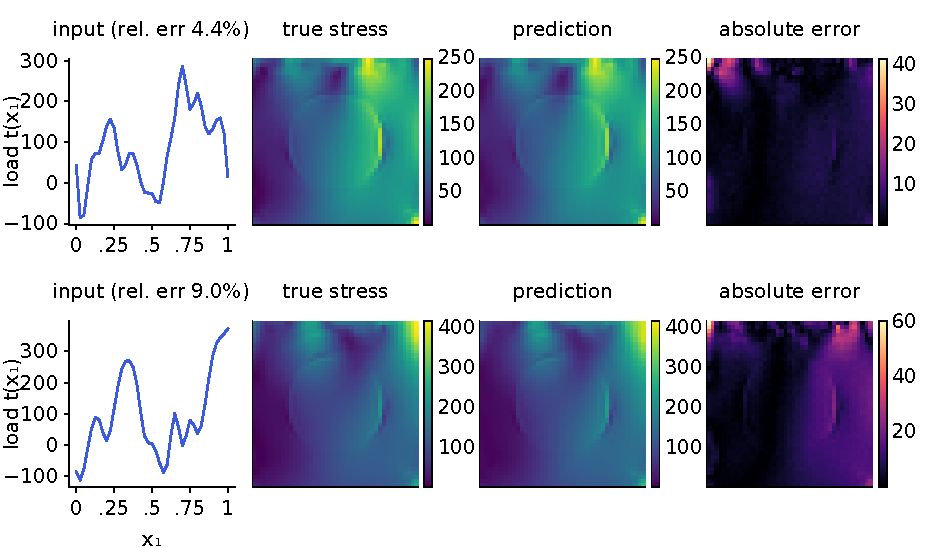
\includegraphics[width=\linewidth]{figs/fields.pdf}
\caption{Example predictions of the full pipeline. Top: a median-error test
case; bottom: a case at the 98th error percentile. Columns: input load, true
von Mises stress, prediction, and pointwise absolute error; the error panels
use a smaller scale. Errors concentrate in the high-traction corner, as also reported by
\citet{mora2025operator}.}
\label{fig:fields}
\end{figure}
\subsection{Training Variability and Test-Sample Uncertainty}
\label{sec:uncertainty-budget}
The seed standard deviations measure training and selection variability on a fixed test block. Separately, the observed per-case standard deviation $0.0169$ gives a standard error of about $\seTest$ percentage points for the mean over 20000 i.i.d. cases, conditional on a fixed predictor. The published comparison provides neither per-case predictions nor retraining variability, so no significance or equivalence test against PARA-Net is available. Within-study comparisons use paired per-case differences, and their seed spreads describe sensitivity to retraining.

The public test blocks have been used repeatedly across the benchmark
analyses. Reported intervals and paired differences are descriptive of
these cases and do not adjust for repeated test-set analysis. The
fixed-predictor sampling calculations and conformal guarantees require
the independence and exchangeability assumptions stated with each result.

\subsection{Architectural Diversity and the Shared Residual}
\label{sec:diversity}
The uncentered normalized-residual alignments
$S_{ij}/\sqrt{S_{ii}S_{jj}}$ range from $\corrNetLoSix$ to
$\corrNetHiSix$ across the six-member experiment, with mean
$\corrBarSix\pm\corrBarSixSd$. The exact ensemble identity uses the
second-moment matrix $S$ itself. Centered residual correlations are shown
separately in Supplement Figure~\ref{fig:corr}.

For each seed, we estimate $S$ on validation and minimize $w^\top Sw$ over the simplex. The resulting validation RMS errors are $\predRMS\pm\predRMSSd\%$ for five members and $\predRMSSix\pm\predRMSSixSd\%$ for six. The dispersion factors $\dispFac\pm\dispFacSd$ and $\dispFacSix\pm\dispFacSixSd$ compare the mean and RMS errors of the same fitted mixture on that same validation set. For six members, the test-mean/validation-RMS ratio is approximately $0.936\pm0.011$; this ratio combines metric dispersion and transfer between samples.

The equicorrelation references $\ensFloor\%$ for five members and
$\ensFloorSix\%$ for six use average member RMS errors, together with
average centered correlations in the five-member calculation and average
uncentered alignments in the six-member calculation. Both are descriptive
approximations for these heterogeneous pools. The rigorous entrywise lower
bounds of Corollary~\ref{cor:floor} are computed directly from the measured
matrix in Section~\ref{sec:theory-secmom}.

The across-member mean residual accounts for about 90\% of average residual energy on validation and concentrates near the corners of the loaded edge. It has more high-frequency energy than the target fields, and leading residual directions align across architectures (Online Appendix~1, Section~\ref{supp:experiments}). These observations identify shared structured error in the trained pool. Its cause remains unresolved: common surrogate bias and finite-element or interpolation effects are both possible. Because the target is a deterministic numerical map, solver discrepancy relative to a continuum solution is not by itself irreducible error for learning the numerical labels.

Learning curves show modest additional gains over the tested data range: the normalized-MSE model moves from $\lcMlpEightK\pm\lcMlpEightKSd\%$ at 8000 fitting rows to $\lcMlpNineteenK\pm\lcMlpNineteenKSd\%$ at 19000. Online Appendix~1, Section~\ref{supp:experiments} contains the learning curves, residual plots, ablations, and cost measurements.

\subsection{Seed and Architecture Diversity}
\label{sec:seeds-arch}
The sixty-member analysis uses ten seeds of six model configurations, treating these configurations as blocks. The public test block is split into 1000 calibration cases for fitted weights and 19000 evaluation cases; hindsight optima are explicitly computed on evaluation. The RMS-optimal global convex mixture attains $\saSixtyOracleRms\%$ RMS error and $\saSixtyOracle\%$ mean error. The latter is the mean error of the RMS-optimal weights, not a minimum of the mean-error objective.

Theorem~\ref{thm:blockfloor}, applied to the evaluation matrix and its smallest within- and between-block entries, gives $\saBound\%$ RMS as an empirical lower bound for every global convex combination of these sixty predictors on these cases. The gap to the empirical optimum is approximately $0.063$ percentage points. The bound concerns global convex combinations of these sixty predictors; per-pixel affine and kernel-corrected estimators lie outside its class.

The deployed six-member corrected pipeline has mean error $\saDeployedEv\pm\saDeployedEvSd\%$ on the same evaluation cases. This is below the mean error of the RMS-optimal convex mixture. The pipeline fitted to the six ten-seed mean predictors reaches $\saPoolPipeline\%$, a gain outside the theorem's estimator class. Table~\ref{tab:seedarch} lists the fitted-stack comparisons in both metrics.

\begin{table}[t]
\centering

\begin{adjustbox}{max width=\linewidth}
\begin{tabular}{lcc}
\toprule
Pool and weights & Error (\%) & RMS (\%) \\
\midrule
FNO, one seed & \saFnoOne & \saFnoOneRms \\
FNO, ten seeds, equal weights & \saFnoTen & \saFnoTenRms \\
Six architectures, one seed, equal weights & $\saSixEq\pm\saSixEqSd$ & $\saSixEqRms\pm\saSixEqRmsSd$ \\
Six architectures, one seed, convex, fitted & $\saSixConvex\pm\saSixConvexSd$ & -- \\
Sixty, equal weights & \saSixtyEq & \saSixtyEqRms \\
Sixty, convex, fitted & \saSixtyConvex & \saSixtyConvexRms \\
Sixty, convex, hindsight & \saSixtyOracle & \saSixtyOracleRms \\
Lower bound of Theorem~\ref{thm:blockfloor} on the sixty & -- & \saBound \\
Six ten-seed means, per-pixel affine, fitted & \saPerpixMeans & -- \\
Sixty, per-pixel affine, leave-one-out ridge, fitted & \saPerpixSixtyLoo & -- \\
Six means and the learned kernel, per-pixel affine, leave-one-out ridge & \saSevenMeansLoo & -- \\
Six ten-seed means, per-pixel affine and kernel correction, fitted & \saPoolPipeline & -- \\
Deployed six-member pipeline, one seed & $\saDeployedEv\pm\saDeployedEvSd$ & -- \\
\bottomrule
\end{tabular}
\end{adjustbox}
\caption{Sixty predictors, ten seeds of six architectures, on the evaluation
subset of the test block ($19000$ cases). Mean relative $L^2$ error, and the
root-mean-square relative error used in the ensemble bounds. Convex weights are
fitted on the disjoint calibration subset ($1000$ cases) unless marked
hindsight, where they are chosen on the evaluation subset itself. Rows with
$\pm$ are means over the ten seeds.}
\label{tab:seedarch}
\end{table}
\subsection{Uncertainty Quantification}
\label{sec:uq}
The single-mean power-function bound and its correction-label mismatch extension appear in Section~\ref{sec:theory-or}. Section~\ref{sec:implementation-sensitivity} measures the propagated mismatch; the residual RKHS norm itself is not observed, so the bound is not evaluated numerically. Fitted-function norms are computable diagnostics: the squared-norm ratio is about 4900 before normalizing target energy and about 8.8 after it (Table~\ref{tab:norms}).

The power function has weak correlation with the absolute error ($\uqCorrAbs$) and negative correlation with relative error, while correlating with output norm ($\uqCorrNorm$). Disagreement is similarly weak as an error indicator ($\uqDisAbs\pm0.006$ against absolute error). Agreement among predictors cannot reveal an error component shared identically by all of them, and neither scale ranks the error well here.

For the six-member pipeline, conformal calibration on 1000 cases and evaluation on the disjoint 19000 give $\uqPlamSix\pm\uqPlamSixSd\%$ coverage at nominal 90\% and $\uqPlamSixHi\pm\uqPlamSixHiSd\%$ at nominal 95\%. Under the frozen-predictor i.i.d. continuous-score assumptions of Remark~\ref{rem:covlaw}, the corresponding central 95\% reference intervals are $[88.0\%,91.8\%]$ and $[93.5\%,96.3\%]$; all ten seeds lie inside each.

A constant-radius conformal set gives $\uqRawSix\pm\uqRawSixSd\%$ and $\uqRawSixHi\pm\uqRawSixHiSd\%$ coverage and is narrower on average: the power-function set has mean radius $\uqWidthRatio$ times as large. The power-function set also varies markedly across deciles, from 69\% to 99.9\% coverage at seed zero. Thus marginal coverage is compatible with poor local coverage and weak error ranking. Online Appendix~1, Section~\ref{supp:experiments} includes all three scales and the five-member comparisons. The coverage guarantee and its assumptions are stated in Section~\ref{sec:theory-conf}.

\subsection{Sensitivity to Centering and Correction Labels}
\label{sec:implementation-sensitivity}
Two paired experiments examine the distinction between the training-row
kernel predictions and the predictor evaluated at a new input. First, we
compare the six-member pipeline at the same ten seeds, changing only the
target mean used in each out-of-fold kernel fit. Both arms retrain the
kernel-conditioned refiner for 100 epochs and refit the stack and residual
correction; the remaining members are held fixed. Pooled centering gives
$\sensPooled\pm\sensPooledSd\%$ mean relative error and fold-local
centering gives $\sensLocal\pm\sensLocalSd\%$. The paired difference,
fold-local minus pooled, is $\sensCenterDelta\pm\sensCenterDeltaSd$
percentage points. Figure~\ref{fig:implementation-sensitivity} shows the
paired changes at every seed.

Second, we hold the stack weights and selected correction kernel
fixed, evaluate the query-time mean on the training rows, and replace the
correction labels by residuals of that mean. The neural networks remain fixed. The resulting test error is
$\sensConsistent\pm\sensConsistentSd\%$, a paired change of
$\sensMismatchDelta\pm\sensMismatchDeltaSd$ percentage points from the
original correction. The propagated mismatch
$\|c_\lambda(u)^\top\Delta\|_2/\|G(u)\|_2$ from
\eqref{eq:mismatch} averages
$\sensMismatchMean\pm\sensMismatchMeanSd\%$ across seeds and cases.
It measures the difference between two finite-design predictors.
Online Appendix~1, Section~\ref{supp:sensitivity} gives the protocol, paired pipeline comparisons,
and calibration results.

\begin{figure}[t]
\centering
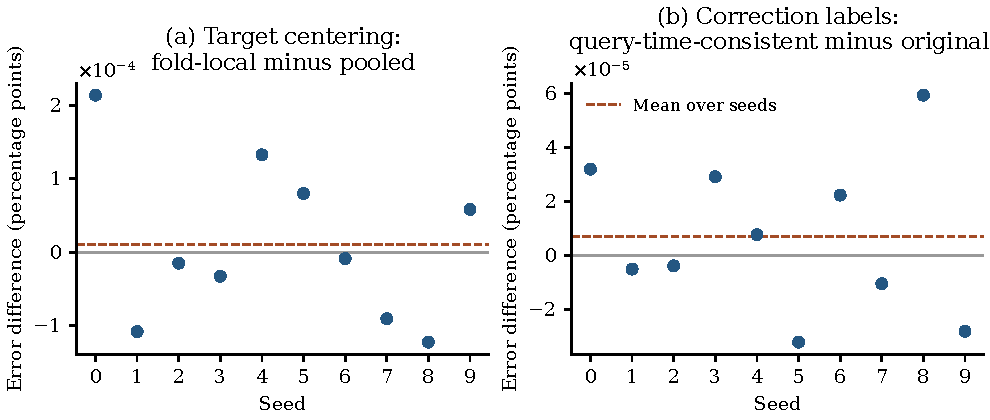
\includegraphics[width=\linewidth]{figs/paired_implementation_sensitivity.pdf}
\caption{Paired changes in mean relative test error for the ten mechanics
seeds. Left: fold-local minus pooled target centering, with downstream
refiner training and fitting repeated in both arms. Right: correction labels
consistent with the query-time mean minus the original labels, with the
mean and kernel fixed. Positive values mean higher error after the change.
The panels use separate vertical scales. All points use the same public
test block; the dashed lines are seed means.}
\label{fig:implementation-sensitivity}
\end{figure}


\section{The OCO-2 Radiative-Transfer Emulator}
\label{sec:oco2}
On structural mechanics, residual kernel correction gives a small,
repeatable improvement to the stacked predictor. The OCO-2 experiments
examine neural-feature kernel readouts for the radiative-transfer emulation
problem of \citet{susiluoto2025radiative}. For each spectral band of the
OCO-2 instrument, the task is to learn the map from a reduced
atmospheric state ($20$--$24$ dimensions after the dimension reduction of
that paper) to the reduced radiance ($40$ PCA coefficients of the
monochromatic spectrum). The OSF project (\texttt{u2t8a}) publishes a training
pool of $20000$ pairs and, separately, $2000$ test states together with the
kernel-flow emulator's own predictions on them; the training and test sets share no point. We split the pool
$18000/2000$ into training and validation. Within each run, the validation
split selects network checkpoints, kernel length scales and nuggets, and
the coordinatewise model selections below. The public test states are used for the reported
evaluation. Section~\ref{sec:oco-grid-sensitivity} reports a separate
matched sensitivity experiment.
The validation subset comes from the source study's Sobol training design,
whereas the public test states are a separate draw. The flat network's mean
relative error is $6.7\%$ on validation and $4.4\%$ on test for O2,
indicating a material difference between the two evaluation sets.
All comparisons with the published emulator use identical test points.

The two error criteria are defined here on the released reduced
representation. Neither is the source study's instrument-noise or retrieval
acceptance test. Let $z\in\mathbb R^{40}$ contain the standardized
coefficients, let $U$ have the retained orthonormal PCA columns, and put
$D_z=\operatorname{diag}(s_z)$. The stored means and scales reconstruct
\begin{equation}
 R(z)=\mu_y+U(\mu_z+D_z z),\qquad U^\top U=I.
 \label{eq:oco-reconstruction}
\end{equation}
The two reported mean relative errors are
\begin{align}
 E_{\rm red}&=\frac1N\sum_{i=1}^N
       \frac{\|\hat z_i-z_i\|_2}{\|z_i\|_2},
       \label{eq:oco-reduced}\\
 E_{\rm rad}&=\frac1N\sum_{i=1}^N
       \frac{\|D_z(\hat z_i-z_i)\|_2}{\|R(z_i)\|_2}.
       \label{eq:oco-radiance}
\end{align}
Orthogonality gives $\|R(\hat z)-R(z)\|_2
=\|D_z(\hat z-z)\|_2$; the reconstruction offsets cancel in the
numerator but remain in the denominator. The radiance criterion compares
two forty-component reconstructions, so it excludes PCA truncation error,
the instrument line shape, and the measurement-noise model. Its numerator
weights concentrate on the leading coefficients.

For fixed nonnegative weights $\omega_i,a_j$, the squared objective
$N^{-1}\sum_{i,j}\omega_i a_j(\hat z_{ij}-z_{ij})^2$ separates by
coordinate. Ordinary coordinatewise RMSE selection minimizes this
objective with $\omega_i=a_j=1$. Squared relative coefficient error instead
uses $\omega_i=\|z_i\|_2^{-2}$; squared relative radiance error uses
$\omega_i=\|R(z_i)\|_2^{-2}$ and $a_j=s_{z,j}^2$. Fixed per-sample
denominators therefore preserve separability for the squared objectives,
although they can change the selected member. The square root in each
summand of \eqref{eq:oco-reduced}--\eqref{eq:oco-radiance} couples
coordinates, so coordinatewise selection need not minimize either reported
mean norm, or both simultaneously.

\begin{table}[t]
\centering

\begin{adjustbox}{max width=\linewidth}
\begin{tabular}{lcc}
\toprule
model & reduced & radiance \\
\midrule
Mat\'ern kernel, raw input, one length scale & $40.57\pm0.10$\% & $0.233\pm0.003$\% \\
Mat\'ern kernel, raw input, sensitivity-scaled (ARD) & $29.98\pm0.15$\% & $0.204\pm0.087$\% \\
kernel-flow emulator \citep{susiluoto2025radiative} & 16.89\% & 0.0448\% \\
residual MLP, flat metric & $4.43\pm0.05$\% & $0.195\pm0.014$\% \\
residual MLP, weighted-coefficient loss & $49.32\pm0.40$\% & $0.0442\pm0.0044$\% \\
residual MLP, exact radiance loss & $59.02\pm0.76$\% & $0.0571\pm0.0057$\% \\
Mat\'ern head on the flat network's features & $4.11\pm0.05$\% & $0.0793\pm0.0072$\% \\
Mat\'ern head on the weighted network's features & $21.70\pm0.52$\% & $0.0319\pm0.0020$\% \\
Mat\'ern head on the radiance network's features & $20.48\pm0.61$\% & $0.0379\pm0.0037$\% \\
per-coordinate combination & $\mathbf{4.12\pm0.05}$\% & $\mathbf{0.0294\pm0.0020}$\% \\
\bottomrule
\end{tabular}
\end{adjustbox}
\caption{OCO-2 O2 band, scored on the $2000$ public test states, which are
disjoint from the training pool; within-run selection used a validation
split of the pool. Each fitted-model row is mean $\pm$ standard deviation over ten
seeds; neural networks use a matched $250$-epoch budget. The
kernel-flow row is the emulator of \citet{susiluoto2025radiative}, scored
from its own stored predictions on fixed test points, and is identical at
every seed. ``Features'' means the penultimate
activations of the trained network; the kernel head uses exact
Mat\'ern regression, and the two raw-input rows
are fit by that same kernel-tuning routine and budget as the feature heads:
the same scale grid $\{0.5,1,2,4\}$ times the median distance, the same
nugget grid $\{10^{-8},10^{-6},10^{-4}\}$, the same $6000$-sample tuning
subsample, and the selected kernel refit on all $18000$ training points. This matches the kernel stage; feature heads additionally require neural-network training. The
raw-input rows' selected settings vary from seed to seed; every feature head,
by contrast, selected the largest multiplier ($4$) and the smallest nugget
($10^{-8}$) of that grid at all thirty combinations of band and seed, so the feature-head
numbers are tied to this search grid; Section~\ref{sec:oco-grid-sensitivity}
examines a wider one. The ARD radiance summary includes a bimodal selection
outcome: configurations selected on reduced validation error give
$0.150\%$ radiance error at seven seeds and $0.329\%$ at three.}
\label{tab:oco2}
\end{table}

\begin{table}[t]
\centering

\begin{adjustbox}{max width=\linewidth}
\begin{tabular}{lcc}
\toprule
model & reduced & radiance \\
\midrule
\multicolumn{3}{l}{\emph{O2 band} (10 seeds)} \\
network, flat loss & $4.43\pm0.05$\% & $0.195\pm0.014$\% \\
\quad ridge readout on its frozen features & $4.71\pm0.07$\% & $0.228\pm0.014$\% \\
\quad Mat\'ern head on its frozen features & $4.11\pm0.05$\% & $0.0793\pm0.0072$\% \\
network, weighted-coefficient loss & $49.33\pm0.40$\% & $0.0439\pm0.0031$\% \\
\quad ridge readout on its frozen features & $45.71\pm0.61$\% & $0.0521\pm0.0043$\% \\
\quad Mat\'ern head on its frozen features & $21.72\pm0.52$\% & $0.0316\pm0.0019$\% \\
\multicolumn{3}{l}{\emph{WCO2 band} (10 seeds)} \\
network, flat loss & $16.44\pm0.06$\% & $0.226\pm0.012$\% \\
\quad ridge readout on its frozen features & $16.51\pm0.06$\% & $0.252\pm0.017$\% \\
\quad Mat\'ern head on its frozen features & $16.28\pm0.06$\% & $0.116\pm0.007$\% \\
network, weighted-coefficient loss & $62.57\pm0.56$\% & $0.0738\pm0.0057$\% \\
\quad ridge readout on its frozen features & $61.32\pm0.43$\% & $0.0842\pm0.0067$\% \\
\quad Mat\'ern head on its frozen features & $48.67\pm0.45$\% & $0.0533\pm0.0054$\% \\
\multicolumn{3}{l}{\emph{SCO2 band} (10 seeds)} \\
network, flat loss & $8.23\pm0.02$\% & $0.199\pm0.015$\% \\
\quad ridge readout on its frozen features & $8.33\pm0.03$\% & $0.236\pm0.032$\% \\
\quad Mat\'ern head on its frozen features & $8.08\pm0.01$\% & $0.109\pm0.007$\% \\
network, weighted-coefficient loss & $36.46\pm0.65$\% & $0.0751\pm0.0025$\% \\
\quad ridge readout on its frozen features & $40.10\pm0.91$\% & $0.0866\pm0.0039$\% \\
\quad Mat\'ern head on its frozen features & $15.47\pm0.47$\% & $0.0631\pm0.0037$\% \\
\bottomrule
\end{tabular}
\end{adjustbox}

\caption{Readout control for the kernel heads, ten seeds per band, mean
$\pm$ standard deviation over seeds. For the flat and weighted-coefficient
networks the same
frozen last-layer features are compared under three readouts: the network's own
trained output layer, a ridge regression refit on those features with
the penalty chosen on validation, and the exact Mat\'ern head. The network and kernel-head results are from a separate readout-control experiment. Small differences from
Table~\ref{tab:oco2} reflect repeated network training under the same
seed and split protocol; Online Appendix~1, Section~\ref{app:impl} gives its training protocol.}
\label{tab:oco2ridge}
\end{table}

\begin{figure}[t]
\centering
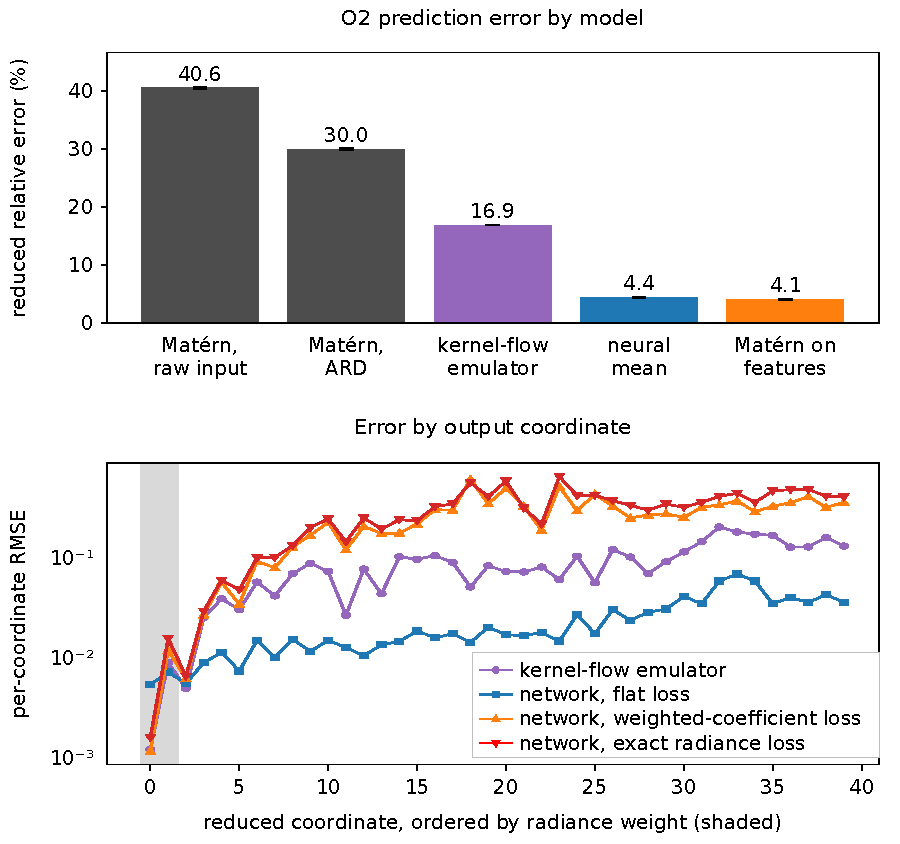
\includegraphics[width=\linewidth]{figs/oco2_seeded.pdf}
\caption{O2 results over ten seeds. Upper panel: reduced error for the
representation comparison; bars and error bars are seed means and standard
deviations. Exact Mat\'ern regression has $40\%$ error on raw inputs and
$4.1\%$ on the trained network's features; the kernel-flow emulator and the
network have intermediate reduced errors. Lower panel: per-coordinate test
RMSE averaged over seeds, with coordinates ordered by their radiance weight
(shaded). Networks are named by their training loss. The coordinate combination
selects each output by validation RMSE.}
\label{fig:oco2}
\end{figure}

The per-output-tuned kernel-flow emulator is more accurate than the flat
network on the heavily weighted leading coefficient ($0.0012$ against
$0.0054$), while the flat network is nearly four times more accurate across
the trailing thirty coordinates, which have small radiance weights
($0.0276$ against $0.1037$). Both weighted losses reduce leading-coefficient
RMSE to comparable values ($0.0012$ and $0.0016$) while increasing error in
the trailing coefficients.

Table~\ref{tab:oco2} and Figure~\ref{fig:oco2} show the principal comparisons.
The fitted kernel has reduced test error $40\%$ on raw input, $30\%$ after rescaling
each input coordinate by its estimated sensitivity, and $4.1\%$ on the
trained network's features. Under this routine, learned features are more
useful than the raw coordinates or the tested input rescaling. The deep
kernel head is the most accurate single predictor on the O2 reduced metric
in this $250$-epoch comparison.
Its error and the error of the network supplying its features are $4.11\pm0.05\%$ against
$4.43\pm0.05\%$, and the head has lower error at all ten seeds
on each band.

A linear ridge regression refitted on the same frozen features
(Table~\ref{tab:oco2ridge}) is worse than the network's trained output layer
on the flat-loss network for every combination of band and seed. The Mat\'ern head is better
than both for every combination of band and seed, with a margin over ridge of
$0.60\pm0.07$ percentage points on O2 and about a quarter of a point on
the other bands. Thus the linear-refit control does not reproduce
the Mat\'ern improvement. Adding the ridge readouts to coordinate selection
changes the combination by at most $0.002$ percentage points on any band.

The combination row is produced by the unweighted selector over the three networks and
their three feature-kernel heads. It takes each reduced
coordinate from the model with the smallest validation root-mean-square
error on that coordinate. A second selector weights observations by the
inverse squared norm of each validation state. By
Corollary~\ref{cor:percoordw}, it exactly minimizes the empirical squared
relative error over the coordinatewise candidate choices. The weighted
selector chooses different models at three seeds on O2 and four on WCO2,
but changes each band's mean reduced error by less than $0.001$ percentage
points, with unchanged radiance means at the reported precision. On O2 the unweighted combination has mean
reduced error $4.11510\%$, slightly above the flat-feature head's
$4.11080\%$, while improving radiance error from $0.07927\%$ to
$0.02940\%$. It therefore does not dominate every individual model on both
criteria.

Uncertainty in the comparison with the emulator is assessed using paired predictions: on the same $2000$ test states,
a case-resampling bootstrap of the difference between the combination and
the emulator excludes zero at ten of ten seeds on both metrics on O2 and
SCO2, and at ten of ten on WCO2's reduced metric and nine of ten on its
radiance metric, the exception being the seed with higher error by $0.0015$ points;
the seed standard deviations in Table~\ref{tab:oco2} describe retraining variability. The comparison concerns the two criteria defined here on the released
reduced representation (the coefficients, and the radiance reconstructed from the retained forty components), with the networks at a $250$-epoch
budget and the emulator fitted on $20000$ states against our $18000$ plus a
$2000$-state validation subset. Instrument response, Jacobians and the
retrieval itself are outside its scope.

A separate O2 experiment compares
isotropic, learned diagonal, and low-rank Mahalanobis metrics using the
kernel-flows loss of \citet{owhadi2019kernel}. The learned diagonal metric
has approximately $30\%$ reduced error on raw states, and the low-rank
extension does not improve it. Learned metrics also give no improvement
over the isotropic kernel in that experiment's separate neural-feature
representation. Online Appendix~1, Section~\ref{supp:oco-learned-metric} specifies this
experiment's 6000-row kernel budget and its feature-training protocol;
it is distinct from the matched comparisons in Table~\ref{tab:oco2}.

\subsection{Input Metric and Kernel Accuracy}
\label{sec:aniso-measured}
A sweep refits both raw-input kernel rows at five nested
training sizes, ten seeds per band, estimating the sensitivity map from
the available training rows at each size. At $n=18000$ the isotropic-to-adapted
error ratios range from $1.1$ to $1.5$. The fitted log--log slopes differ
little on O2 and more on strong CO$_2$; the numerical results are in
Section~S7. These slopes summarize a finite range of training sizes.
Proposition~\ref{prop:aniso} gives a finite-design bound for rank
truncation under Lipschitz and native-space assumptions.
\subsection{Transfer of the Two-Member Rule}
\label{sec:secmom-margin}
Part~(i) of Proposition~\ref{prop:secmom} says that a weaker member helps
the optimal two-member squared-relative-error mixture exactly when
$\varrho<e_1/e_2$. We examine this criterion using stored
validation and test predictions for eight models: the two raw-input
kernels, three networks, and three feature-kernel heads. There are
$\binom{8}{2}=28$ pairs for each of thirty combinations of band and seed, $840$ in all.

When estimated on the same block, the criterion correctly identifies
whether the optimal convex mixture improves on the better member for all $840$ pairs.

To assess transfer, we estimate $\varrho$ and $e_1/e_2$ on validation
and compare the resulting decision with the test-block result.
The test-side outcome is
whether the optimal convex two-member mixture improves on the better of the two members
\emph{on test}, whichever that is (the order of a pair flips between the
splits in $40$ of the $840$). The rule is correct on $62.4\%$ of the $840$
pairs. Stratified by the observed margin
$|\varrho-e_1/e_2|$ that the rule must resolve, the outcome is
$101$ of $257$ below $0.02$, $95$ of $215$ from $0.02$ to $0.05$, $81$ of
$88$ from $0.05$ to $0.10$, $215$ of $248$ from $0.10$ to $0.25$, and $32$
of $32$ above $0.25$ --- that is $39\%$, $44\%$, $92\%$, $87\%$ and
$100\%$. These counts assess the existence of an improving convex mixture. Scoring instead the
mixture at the weight fitted on validation, against the better test member,
the counts are $142$ of $257$, $107$ of $215$, $76$ of $88$,
$125$ of $248$ and $31$ of $32$ ($57.3\%$ overall). These counts measure agreement between
the rule and the performance of the transferred mixture; in
absolute terms $356$ of the $840$ transferred mixtures improve on the better test
member, all of them among the $715$ pairs with a positive inclusion decision.
The existence of an improving mixture does not ensure that a weight
fitted on validation achieves that improvement on test. The
calculations use the root-mean-square relative error and
uncentered alignment of the proposition
(\texttt{oco\_ensemble\_recheck.json} in the release). The $28$ pairs for each band and seed share members and the ten seeds of a band
share one test block, so the bins describe a trend across margin rather
than binomial samples. The rule transfers poorly between validation and test on pairs with small margins.

The signed gap $D=\varrho-e_1/e_2$ changes between validation and test
with empirical standard deviation $0.099$ across these dependent pairs and
mean change $0.0004$. Its within-pair seed scatter is $0.010$. The
difference between the validation and test designs is therefore material in this diagnostic;
Proposition~\ref{prop:margin} turns such a shift into a probabilistic bound
under an estimation-error condition, and the margin bins describe this pool.

For the raw-input kernel against the flat network, the ten-seed validation
means are $\varrho=0.156$ and $e_n/e_k=0.157$. The difference changes sign
across seeds, giving an inclusion decision at five of ten. The corresponding
optimal validation RMS relative errors are $8.4079\%$ for the mixture and
$8.4081\%$ for the network, at a network weight of $0.9999$. The test-block
hindsight optimum differs from the network by $0.0004$ percentage points.
These gains are too small to support a practical improvement from this
pair, which accounts for its limited contribution.

\subsection{Data Scaling}
\label{sec:oco-scaling-summary}
The OCO-2 error decreases over the training sizes examined. The learning
curves and the large-$n$ ClimSim results are reported in Section~S7.

\subsection{Sensitivity to the Kernel Search Grid}
\label{sec:oco-grid-sensitivity}
The boundary selections in Table~\ref{tab:oco2} motivate expanding
the search range. For each band, we compare two kernel grids on fixed neural predictions
and features trained at seeds 0, 1, and 2. The original grid has 12 scale--nugget pairs;
the expanded grid has 56. Both searches use the same validation objective,
6000-row tuning subset, and full-training refit. The raw-input, ARD-input
and three feature kernels receive the same expanded candidates. Network
training remains at 250 epochs. This three-seed comparison uses networks trained separately from those
in the ten-seed experiment.

Table~\ref{tab:oco-grid-sensitivity} reports representative predictors
under both searches. Expanding the grid changes the validation-selected
hyperparameters, with both increases and decreases in test error across
seeds. For the coordinate combination, mean reduced
error rises from $\sensOtwoComboOldRed\%$ to $\sensOtwoComboNewRed\%$ on O2,
from $\sensWcoComboOldRed\%$ to $\sensWcoComboNewRed\%$ on WCO2, and from
$\sensScoComboOldRed\%$ to $\sensScoComboNewRed\%$ on SCO2. The radiance
changes have mixed signs across seeds. The flat-feature kernel head
outperforms the raw-input kernel on the reduced criterion in each band.
Online Appendix~1, Section~\ref{supp:sensitivity}
gives results for all fourteen predictors, paired differences, boundary selections,
and counts of numerical failures.

\begin{table}[t]
\centering

\begin{adjustbox}{max width=\linewidth}
\begin{tabular}{llcccc}
\toprule
& & \multicolumn{2}{c}{Reduced error (\%)} & \multicolumn{2}{c}{Radiance error (\%)} \\
\cmidrule(lr){3-4}\cmidrule(lr){5-6}
Band & Model & Original grid & Expanded grid & Original grid & Expanded grid \\
\midrule
O2 & Raw input & $40.529\pm0.089$ & $40.529\pm0.089$ & $0.2353\pm0.0047$ & $0.2353\pm0.0047$ \\
O2 & ARD input & $30.019\pm0.035$ & $29.062\pm0.165$ & $0.2706\pm0.1030$ & $0.1519\pm0.0007$ \\
O2 & Flat-loss network & $4.440\pm0.087$ & $4.440\pm0.087$ & $0.1893\pm0.0158$ & $0.1893\pm0.0158$ \\
O2 & Flat-feature head & $4.104\pm0.074$ & $4.331\pm0.074$ & $0.0821\pm0.0092$ & $0.1260\pm0.0203$ \\
O2 & Coordinate combination & $4.112\pm0.068$ & $4.329\pm0.075$ & $0.0282\pm0.0012$ & $0.0285\pm0.0012$ \\
\addlinespace
WCO2 & Raw input & $58.625\pm0.202$ & $58.625\pm0.202$ & $0.4431\pm0.0063$ & $0.4431\pm0.0063$ \\
WCO2 & ARD input & $52.454\pm0.071$ & $53.505\pm0.073$ & $0.2231\pm0.0014$ & $0.7523\pm0.0106$ \\
WCO2 & Flat-loss network & $16.419\pm0.070$ & $16.419\pm0.070$ & $0.2268\pm0.0049$ & $0.2268\pm0.0049$ \\
WCO2 & Flat-feature head & $16.270\pm0.067$ & $16.395\pm0.073$ & $0.1154\pm0.0012$ & $0.1770\pm0.0046$ \\
WCO2 & Coordinate combination & $16.270\pm0.068$ & $16.393\pm0.072$ & $0.0537\pm0.0069$ & $0.0544\pm0.0056$ \\
\addlinespace
SCO2 & Raw input & $41.012\pm0.090$ & $43.708\pm0.065$ & $0.5229\pm0.0081$ & $0.5738\pm0.0054$ \\
SCO2 & ARD input & $28.717\pm0.021$ & $28.717\pm0.021$ & $0.6023\pm0.0097$ & $0.6023\pm0.0097$ \\
SCO2 & Flat-loss network & $8.236\pm0.021$ & $8.236\pm0.021$ & $0.2060\pm0.0209$ & $0.2060\pm0.0209$ \\
SCO2 & Flat-feature head & $8.092\pm0.018$ & $8.108\pm0.025$ & $0.1094\pm0.0051$ & $0.1142\pm0.0093$ \\
SCO2 & Coordinate combination & $8.091\pm0.018$ & $8.107\pm0.025$ & $0.0573\pm0.0045$ & $0.0566\pm0.0033$ \\
\bottomrule
\end{tabular}

\end{adjustbox}
\caption{OCO-2 search-grid sensitivity, three paired seeds per band.
Entries are mean $\pm$ sample standard deviation, in percent. Each pair
uses the same trained networks and validation split. The source emulator
and linear-readout controls, together with every feature head and both
coordinate selectors, appear in Online Appendix~1, Section~\ref{supp:sensitivity}.}
\label{tab:oco-grid-sensitivity}
\end{table}


\section{Theory}
\label{sec:theory}
Throughout this section $\mathcal U=\mathbb R^p$ denotes the (discretized) input
space and $\mathcal V=\mathbb R^q$ the output space, $G:\mathcal U\to\mathcal V$
the target operator, $\mu$ the input distribution, and
$(u_1,v_1),\dots,(u_N,v_N)$ i.i.d.\ draws with $v_n=G(u_n)$; the labels have no
observation noise because they come from a deterministic solver;
Section~\ref{sec:diversity} discusses solver error. Assume $\|G(u)\|_2>0$ almost surely and that all displayed expectations are finite. We write
$\ell(w,v)=\|w-v\|_2/\|v\|_2$ for the relative error and
$R(\widehat G)=\mathbb E_{u\sim\mu}\,\ell(\widehat G(u),G(u))$ for the risk, which is
the quantity reported in Section~\ref{sec:experiments}. The results below connect
residual alignment to the scope for averaging, and kernel corrections to
conditional error bounds. The analysis uses standard identities and direct extensions
of classical results. The ensemble-floor, sharp kernel-bound, and minimax theorems are
proved below; Online Appendix~1, Section~\ref{app:proofs} also includes these proofs and
those of the remaining results.

\subsection{Guarantees for the Fitted Stages}
\label{sec:theory-stages-summary}

Section~S1 states results for reflection averaging
(Proposition~\ref{prop:sym}), the kernel-flow regularizer
(Proposition~\ref{prop:kf}), and the stack, affine readout, and kernel
selection stages (Propositions~\ref{prop:stack} and~\ref{prop:affine},
Lemma~\ref{lem:select}, and Corollary~\ref{cor:certificate}). The statistical
selection bounds require candidates fixed before an independent validation
sample is drawn. The deployed pipeline uses validation for checkpoint, member, and kernel
selection, so those bounds describe the dependence on class size, sample size, and correction
weights; several are numerically vacuous at our sample sizes.
Lemma~\ref{lem:kappa} gives the uniform correction-weight bound
$\kappa_{\mathrm{an}}=500$ for the stated kernel normalization and nugget.
Theorems~\ref{thm:or} and~\ref{thm:minimax} are deterministic conditional
bounds, whose unknown native-space norms prevent numerical certification.

Split-conformal coverage has a separate requirement: the predictor and
scale must be fixed independently of exchangeable calibration and
evaluation observations.

\subsection{Residual Alignment and Convex Ensembles}
\label{sec:theory-secmom}

Proposition~\ref{prop:stack} bounds weight selection under independent-validation assumptions; it does not imply that mixing improves on a member. For mean squared relative error, this is decided by a second-moment matrix. For a
map $f$ write the \emph{normalized residual} at $u$ as
$\rho_f(u)=\big(f(u)-G(u)\big)/\|G(u)\|_2$, so that
$\ell(f(u),G(u))=\|\rho_f(u)\|_2$.

\begin{proposition}[second-moment identity for convex stacks]\label{prop:secmom}
Let $f_1,\dots,f_M$ be fixed maps and define
$S\in\mathbb R^{M\times M}$ by
$S_{mk}=\mathbb E_{u\sim\mu}\,\langle\rho_{f_m}(u),\rho_{f_k}(u)\rangle$.
For $w$ in the simplex $\Delta^{M-1}$ let $f_w=\sum_m w_mf_m$. Then
\[
\mathbb E_{u\sim\mu}\,\ell\big(f_w(u),G(u)\big)^2\;=\;w^\top S\,w ,
\]
so the mean squared relative error of every convex stack is determined by $S$, and
the best achievable is $\min_{w\in\Delta^{M-1}}w^\top Sw$. In particular:
\begin{enumerate}
\item[(i)] (two members) if $S$ has diagonal $(e_1^2,e_2^2)$ with $0<e_1\le e_2$
and uncentered correlation $\varrho=S_{12}/(e_1e_2)$, mixing in the weaker member
strictly helps if and only if $\varrho<e_1/e_2$, in which case the optimum is
interior with value $e_1^2e_2^2(1-\varrho^2)/(e_1^2+e_2^2-2\varrho e_1e_2)$;
\item[(ii)] (equicorrelated family) if $S_{mm}=e^2$ and $S_{mk}=\varrho\,e^2$
for all $m\neq k$ with $\varrho\ge0$, then
$\min_{w}w^\top Sw=e^2\big(\varrho+(1-\varrho)/M\big)$, attained at uniform
weights and decreasing to $e^2\varrho$ as $M\to\infty$.
\end{enumerate}
\end{proposition}
\noindent\emph{Proof.} See Online Appendix~1, Section~\ref{proof:prop:secmom}.


If a member has zero squared risk, it already attains the minimum zero; ratios involving its error are not used.

Part~(i) is the classical two-member minimum-variance rule, and part~(ii) is
the equicorrelated case of the ambiguity decomposition of ensemble learning
\citep{krogh1995neural}; see \citet{ueda1996generalization} for the
generalization-error form and \citet{brown2005diversity} for a survey. Both
are applied to the estimated $S$ in the experiments.

The identities in this subsection concern squared relative error, whereas
the tables in Sections~\ref{sec:experiments} and~\ref{sec:oco2} report mean
relative error. Remark~\ref{rem:metric} distinguishes the two metrics.

\begin{remark}[the two error metrics]\label{rem:metric}
For a map $f$ write
$\mathcal E_1(f)=\mathbb E\|\rho_f(u)\|_2$ and
$\mathcal E_2(f)=(\mathbb E\|\rho_f(u)\|_2^2)^{1/2}$, the mean and the root
mean square of the per-sample relative error. If $\mathcal E_1=0$, both errors vanish and no ratio is needed; below assume $\mathcal E_1>0$. The tables report
$\mathcal E_1$; Proposition~\ref{prop:secmom} is a statement about
$\mathcal E_2$, since $\mathcal E_2(f_w)^2=w^\top Sw$ by definition. Writing
$X=\|\rho_f(u)\|_2$ and $c_f=(\operatorname{Var}X)^{1/2}/\mathbb EX$,
\[
\mathcal E_2(f)^2-\mathcal E_1(f)^2=\operatorname{Var}X,
\qquad
\mathcal E_1(f)/\mathcal E_2(f)=(1+c_f^2)^{-1/2}\le1 ,
\]
with equality only if the per-sample error is almost surely constant. The
lower bound concerns $\mathcal E_2$,
because only $\mathcal E_2$ is determined by $S$: the map
$w\mapsto w^\top Sw$ is a quadratic form in second moments, whereas
$w\mapsto\mathbb E\|\sum_m w_m\rho_{f_m}(u)\|_2$ depends on the full joint law
of the residuals. Upper bounds transfer downward, since
$\mathcal E_1\le\mathcal E_2$, while lower bounds do not: relating a lower bound from
$S$ to a reported mean error requires the dispersion of the same
predictor. For the structural-mechanics stack the mean is about six percent
below the RMS; for the O2 predictors of Section~\ref{sec:oco2}, the difference
is ten to eleven percent. This conversion depends on the predictor's error dispersion and therefore
varies across predictors.
\end{remark}

Applying part~(i) requires estimating the errors and their correlation.
The reliability of that decision depends on its distance from the threshold
relative to the estimation error. A margin law for threshold rules of this shape
(Proposition~\ref{prop:margin}, Online Appendix~1, Section~\ref{supp:rules}) bounds the
probability that a decision is both wrong and taken at an observed margin
of at least $\tau$ by $\exp(-\tau^{2}/2\sigma^{2})$, with $\sigma$ the
scale specified by the estimation-error assumption. This is a joint
probability bound. The error rate conditional on an observed margin
exceeding $\tau$ is the joint probability divided by
$\mathbb P(|\widehat D|\ge\tau)$, which the proposition does not bound.
Section~\ref{sec:secmom-margin} therefore measures the accuracy of the
rule empirically within each margin bin.

The equicorrelated model is restrictive. A lower bound for convex weights
needs only one-sided bounds on the entries of $S$.

\begin{corollary}[ensembling floor]\label{cor:floor}
If every member satisfies $S_{mm}\ge\bar e^{\,2}$ and every pair satisfies
$S_{mk}\ge\bar\varrho\,\bar e^{\,2}$ with $\bar\varrho\in[0,1]$, then every
convex combination $f_w$ obeys
\[
\mathbb E\,\ell\big(f_w(u),G(u)\big)^2\;=\;w^\top Sw\;\ge\;
\bar e^{\,2}\big(\bar\varrho+(1-\bar\varrho)\,\|w\|_2^2\big)\;\ge\;
\bar e^{\,2}\,\bar\varrho .
\]
No number of additional members with the same error level and mutual
correlations moves the ensemble's root-mean-square relative error below
$\bar e\sqrt{\bar\varrho}$.
\end{corollary}
\noindent\emph{Proof.} See Online Appendix~1, Section~\ref{proof:cor:floor}.


Upper bounds on the same entries give an upper bound on the optimum by
evaluating uniform weights.

\begin{corollary}[bounds for nearly equicorrelated ensembles]\label{cor:floorpinch}
Suppose $\bar e>0$ and, in addition to the hypotheses of Corollary~\ref{cor:floor}, that
$S_{mm}\le\bar e^{\,2}(1+\delta_e)$ for every $m$ and
$S_{mk}\le(\bar\varrho+\delta_\varrho)\,\bar e^{\,2}$ for every $m\neq k$.
Then
\[
\bar\varrho\;\le\;\frac{1}{\bar e^{\,2}}\min_{w\in\Delta^{M-1}}w^\top Sw
\;\le\;\bar\varrho+\delta_\varrho+\frac{1+\delta_e-\bar\varrho-\delta_\varrho}{M}.
\]
The width of the bracket is the normalized off-diagonal entry spread
$\delta_\varrho$ plus a $1/M$ term: when these entrywise spreads are small, the optimal convex risk is localized. The upper bound is obtained by evaluating uniform weights; it does not upper-bound an arbitrary fitted convex combination.
\end{corollary}
\noindent\emph{Proof.} See Online Appendix~1, Section~\ref{proof:cor:floorpinch}.


Applied to a measured matrix $\widehat S$, these are exact empirical bounds on that same design. For the six-member validation matrices, the weak RMS floor $\sqrt{\min_{i\ne j}\widehat S_{ij}}$ is $4.820\pm0.062\%$, the stronger finite-six-member lower bound is $4.849\pm0.060\%$, and the simplex optimum is $4.920\pm0.057\%$ (mean and sample standard deviation over ten seeds). The six-member value near $4.91\%$ obtained from mean uncentered alignments is an equicorrelation diagnostic.

The floor is stated for convex weights, and the deployed stack is not
convex: its per-pixel weights are affine and unconstrained in sign. For
global weights the sign constraint can be removed exactly.

\begin{corollary}[signed stacks]\label{cor:signed}
If $S$ is positive definite, the minimum of $w^\top Sw$ over all $w$ with
$\sum_m w_m=1$, of either sign, is $1/(\mathbf 1^\top S^{-1}\mathbf 1)$,
attained at $w^\star=S^{-1}\mathbf 1/(\mathbf 1^\top S^{-1}\mathbf 1)$; it
is at most the convex minimum, with equality exactly when $w^\star$ has no
negative coordinate.
\end{corollary}
\noindent\emph{Proof.} See Online Appendix~1, Section~\ref{proof:cor:signed}.


On the measured $S$ the two minima differ by at most $0.00052$ percentage points at every
seed and for both member sets, but not because the constraint is slack: the
unconstrained minimizer carries a small negative coordinate at seven seeds of
ten for the six members and at one seed for the five. The effect of allowing signed global weights is
therefore small here. The improvement of the per-pixel stack over the convex
stack ($0.032$ and $0.035$ points in the two experiments) concerns a different estimator class; the global signed-weight comparison does not isolate the effect of signs or intercepts within that class.

A pool can contain several architectures and several seeds of each
architecture. The next bound distinguishes these two sources of diversity.

\begin{theorem}[seeds and architectures]\label{thm:blockfloor}
Let the pool consist of $K$ seeds of each of $M$ architectures, and suppose
$S_{ii}\ge\bar e^{\,2}$ for every member, $S_{ij}\ge\varrho_w\bar e^{\,2}$
for two seeds of the same architecture and $S_{ij}\ge\varrho_b\bar e^{\,2}$
for members of different architectures, with $0\le\varrho_b\le\varrho_w\le1$.
Then every convex combination obeys
\[
\mathbb E\,\ell\big(f_w(u),G(u)\big)^2\;\ge\;\bar e^{\,2}\Big(\varrho_b
+\frac{\varrho_w-\varrho_b}{M}+\frac{1-\varrho_w}{MK}\Big),
\]
with equality at uniform weights when the three inequalities are equalities.
For extended pools satisfying the same entrywise bounds, no number of seeds of one architecture takes the
root-mean-square error below $\bar e\sqrt{\varrho_w}$, no number of seeds of
$M$ architectures takes it below
$\bar e\sqrt{\varrho_b+(\varrho_w-\varrho_b)/M}$, and no pool of any size
takes it below $\bar e\sqrt{\varrho_b}$.
\end{theorem}
\begin{proof}
Let $W_a=\sum_{k=1}^K w_{a,k}$ be the weight assigned to architecture $a$.
Then $\sum_aW_a=1$. Nonnegativity of the weights lets us apply the three
entrywise lower bounds separately:
\begin{align*}
w^\top Sw
&\ge \bar e^{\,2}\left[
 \|w\|_2^2+\varrho_w\left(\sum_aW_a^2-\|w\|_2^2\right)
 +\varrho_b\left(1-\sum_aW_a^2\right)\right]\\
&=\bar e^{\,2}\left[
 \varrho_b+(\varrho_w-\varrho_b)\sum_aW_a^2
 +(1-\varrho_w)\|w\|_2^2\right].
\end{align*}
Cauchy--Schwarz gives $\sum_aW_a^2\ge1/M$ and
$\|w\|_2^2\ge1/(MK)$. Their coefficients are nonnegative, so substitution
proves the bound. Uniform weights make both Cauchy--Schwarz inequalities
equalities. When the entrywise bounds are equalities too, every step is
an equality. The stated limits follow directly, provided the same bounds
hold throughout the enlarged pool.
\end{proof}


At fixed $M$, increasing $K$ reduces only the term $(1-\varrho_w)/(MK)$ in the lower bound. The within-architecture contribution $(\varrho_w-\varrho_b)/M$ persists. Section~\ref{sec:seeds-arch} applies the formula empirically to sixty trained predictors; it does not assume the same inequalities for untrained members.

Differentiating the two-member optimum in Proposition~\ref{prop:secmom}(i)
quantifies the local trade-off between accuracy and correlation.

\begin{proposition}[accuracy--correlation trade-off]\label{prop:exchange}
In the setting of Proposition~\ref{prop:secmom}(i) write $t=e_2/e_1$ and
assume $-1<\varrho<1/t$ (with $t\ge1$), so the optimum is interior. The optimal
two-member risk is $V=e_1^2\,t^2(1-\varrho^2)/(1+t^2-2\varrho t)$, and
\[
\frac{\partial V}{\partial t}
=\frac{2e_1^2\,t\,(1-\varrho^2)(1-\varrho t)}{(1+t^2-2\varrho t)^2}>0,
\qquad
\frac{\partial V}{\partial\varrho}
=\frac{2e_1^2\,t^2(t-\varrho)(1-\varrho t)}{(1+t^2-2\varrho t)^2}>0 .
\]
A change $(\mathrm dt,\mathrm d\varrho)$ in the second member therefore
leaves the optimal risk unchanged to first order exactly when
$\mathrm d\varrho=-(1-\varrho^2)\,\mathrm dt/\big(t(t-\varrho)\big)$: an
improvement of the second member's error by a fraction $\epsilon$ is
cancelled by a rise of $\epsilon(1-\varrho^2)/(t-\varrho)$ in its correlation
with the first.
\end{proposition}
\noindent\emph{Proof.} See Online Appendix~1, Section~\ref{proof:prop:exchange}.


At perfect anticorrelation $\varrho=-1$, cancellation gives zero optimal risk and the derivative in $t$ is zero, so that boundary is excluded above. At the admission threshold $\varrho=1/t$ with $t>1$, the exchange coefficient $(1-\varrho^2)/(t-\varrho)$ tends to $1/t$; it need not be large. The formula is a local sensitivity calculation at an interior point. Online Appendix~1, Section~\ref{supp:experiments} evaluates it at the measured values.

For coordinate-dependent combinations, squared losses with a fixed diagonal metric separate by coordinate (Proposition~\ref{prop:percoord}; proof in Online Appendix~1, Section~\ref{app:proofs}). The same holds after a fixed sample weighting (Corollary~\ref{cor:percoordw}; proof in Online Appendix~1, Section~\ref{app:proofs}). These statements motivate the selector but do not make it simultaneously optimal for the two reported mean relative norms: the square root couples coordinates, and the two criteria also have different sample denominators. Proposition~\ref{prop:selectcoord} gives an independent-validation selection bound (proof in Online Appendix~1, Section~\ref{app:proofs}); the deployed candidates share the validation split. The OCO-2 combination improves on the rescored source emulator in both mean criteria, while the flat feature head is slightly better on the O2 reduced criterion.

\subsection{Input Geometry and Learned Representations}
\label{sec:theory-aniso}

On structural mechanics, the neural mean and the isotropic kernel differ by
less than half a percentage point. On the O2 band, raw-input kernel error is
roughly nine times the network's error. We examine input scaling and learned
features as two possible explanations for this difference.

A sensitivity-based linear transformation improves the raw-input kernel by a factor of about $1.1$--$1.5$ in this study. Proposition~\ref{prop:aniso} in Online Appendix~1, Section~\ref{supp:rules} gives a finite-design bound for a Lipschitz target after a rank-$r$ truncation, with its approximation error explicit; its proof is in Online Appendix~1, Section~\ref{app:proofs}. The result concerns a specified finite design and rank-$r$ approximation.

The representation affects the native-space bounds, which depend on the target's norm in that space. A fixed kernel may approximate targets outside its RKHS, so native-space membership is not a limit on approximation expressivity. Learned features can change the relevant norm and design geometry, but neither change is automatically favorable.

The optimal-recovery bound in Section~\ref{sec:theory-or}
controls the error by $\|G-m\|_{\mathcal H}\cdot P_\lambda$, a product of
the residual's norm in the kernel's native space and a design factor
determined by the kernel, training inputs, and query. Both depend on the
feature map. On O2, the effective dimension of the Mat\'ern Gram matrix,
controlled by Lemma~\ref{lem:deff}, is nearly identical for raw inputs
and learned features: at $n=4000$, a matched median length scale, and a
$10^{-8}$ nugget, the values are $\alignDeffRaw$ and $\alignDeffFeat$,
respectively. This trace does not determine the pointwise design factor.
At the $2000$ test inputs, the median power function of the feature kernel
is lower by a factor of $\alignRatioP$ at the median scale. Their median
values have ratio $\alignRatioPSel$ at multiplier $4$, the value
selected on validation for every feature head.

The fitted norms differ more substantially. Regressing the same outputs through
the two kernels, the squared native-space norm of the kernel fit,
$\operatorname{tr}(\alpha^\top K\alpha)$, is $\alignRatioNorm$ times
smaller on the features than on the raw input at the median scale
($\alignRatioFull$ times on the full $18000$-row block) and
$\alignRatioSel$ times smaller at the selected multiplier ($\alignRatioFullSel$ times on the
full block). We use $\operatorname{tr}(\alpha^\top K\alpha)$ rather than
$\operatorname{tr}(\alpha^\top Y)$, which also includes
$n\lambda\|\alpha\|_F^2$. The ratios describe finite-design fits in the
interpolating regime. For a target in the corresponding RKHS with
compatible labels, the fitted norm is a lower bound on the target norm.
The ratio grows with the kernel scale: it is $\alignRatioLo$ at half the
median length scale and $\alignRatioHi$ at twice it. At a $10^{-4}$
nugget, where ridge regression no longer interpolates, the ratio decreases
sharply and falls below one at the selected multiplier ($\alignRatioHeavy$).
These comparisons use one seed. Both designs are standardized by their
training moments before forming the kernel, as in the fitted kernel heads. At the reported scales and small nugget, the feature
kernel fits the targets with a smaller fitted RKHS norm and has a smaller
pointwise design factor at the median scale. These measurements do not
isolate the contributions of the norm and design factor to prediction error.

The associated feature-kernel function space has a standard pullback description.
Writing $\varphi$ for the feature map and $k$ for the base kernel, the deep
kernel head uses $k_\varphi(x,x')=k(\varphi(x),\varphi(x'))$, the construction
studied as deep kernel learning \citep{wilson2016deep,calandra2016manifold}.

\begin{proposition}[feature pullback]\label{prop:pullback}
The native space of $k_\varphi$ is $\mathcal H_{k_\varphi}=\{f\circ\varphi:
f\in\mathcal H_k\}$ with
$\|g\|_{\mathcal H_{k_\varphi}}=\min\{\|f\|_{\mathcal H_k}: f\circ\varphi=g
\text{ on }\mathcal U\}$. In particular, if the target factors through the
features as $G=h\circ\varphi$ with $h\in\mathcal H_k$, then
$\|G\|_{\mathcal H_{k_\varphi}}\le\|h\|_{\mathcal H_k}$, and the
optimal-recovery bound of Theorem~\ref{thm:or} for the feature-kernel
regression is governed by $\|h\|_{\mathcal H_k}$ rather than by the norm of
$G$ in the raw-input space.
\end{proposition}
\noindent\emph{Proof.} See Online Appendix~1, Section~\ref{proof:prop:pullback}.


The statement is for scalar $f$; for the vector-valued targets of these
experiments it is applied coordinatewise, with the norm the root sum of squares
over output coordinates, which is the norm Theorem~\ref{thm:or} uses.

This is the standard pullback identity for
reproducing kernels \citep{saitoh1997integral,paulsen2016introduction}. The identity specifies the feature-kernel RKHS and the minimum extension norm. It provides no comparison with the raw-input RKHS without additional assumptions. In particular, a linear feature map is itself an input metric transformation. The measured fitted-norm reduction concerns these fitted kernels at the reported scales and nuggets.

\subsection{An Error Bound for the Residual Kernel Correction}
\label{sec:theory-or}

The final stage of the pipeline is kernel ridge regression of the ensemble
residual. The bound below is a vector-valued, residual form of the classical
power-function estimate for kernel interpolation
\citep{wendland2004scattered} and of the optimal-recovery viewpoint of
\citet{owhadi2019operator}. Fix the mean
$m:\mathcal U\to\mathcal V$; $m$ may be any realized map, including
the stacked ensemble, without a sample-independence requirement. We
write $r=G-m$ for the residual operator with components $r_j$, $j=1,\dots,q$. Let $k$ be a positive definite kernel on $\mathcal U$ with
RKHS $\mathcal H_k$, and assume $r_j\in\mathcal H_k$ for all $j$ with
\[
\|r\|_K^2:=\sum_{j=1}^q\|r_j\|_{\mathcal H_k}^2<\infty .
\]
Given inputs $X=(u_1,\dots,u_n)$, Gram matrix $K=k(X,X)$ and nugget
$\lambda\ge 0$, the correction is
$\widehat r_\lambda(u)=k(u,X)\,(K+n\lambda I)^{-1}R$, $R_{nj}=r_j(u_n)$, and the
corrected predictor is $m+\widehat r_\lambda$. Let
\begin{equation}\label{eq:power}
P_\lambda(u)^2\;=\;k(u,u)-k(u,X)\,(K+n\lambda I)^{-1}k(X,u)
\end{equation}
denote the Gaussian process posterior variance with the same nugget.
The nonnegative square root $P_0$ is the classical power function of the
point set $X$.

\begin{theorem}[conditional power-function bound]\label{thm:or}
For every $u\in\mathcal U$ and every $\lambda\ge0$ (for $\lambda=0$ take $K$
positive definite, or read $K^{-1}$ as the pseudoinverse),
\[
\big\|G(u)-m(u)-\widehat r_\lambda(u)\big\|_2\;\le\;\|G-m\|_K\;
\widetilde P_\lambda(u)\;\le\;\|G-m\|_K\;P_\lambda(u),
\]
where
$\widetilde P_\lambda(u)^2=P_\lambda(u)^2-n\lambda\,\|(K+n\lambda
I)^{-1}k(X,u)\|_2^2$. The first inequality is sharp: for every $u$ there is
a residual operator of norm $\|G-m\|_K$ at which it holds with equality, so
$\|G-m\|_K\widetilde P_\lambda(u)$ is the exact worst-case error of the correction
over the ball $\{r:\|r\|_K\le\|G-m\|_K\}$.
\end{theorem}
\begin{proof}
Put $c=(K+n\lambda I)^{-1}k(X,u)$ and
$g_u=k(u,\cdot)-\sum_i c_i k(u_i,\cdot)$.
The reproducing property expresses each component of the error as
$r_j(u)-\widehat r_{\lambda,j}(u)=\langle r_j,g_u\rangle_{\mathcal H_k}$.
Consequently,
\[
\|r(u)-\widehat r_\lambda(u)\|_2^2
\le\sum_j\|r_j\|_{\mathcal H_k}^2\|g_u\|_{\mathcal H_k}^2
=\|r\|_K^2\|g_u\|_{\mathcal H_k}^2.
\]
Since $Kc=k(X,u)-n\lambda c$, expansion of the squared norm gives
\[
\|g_u\|_{\mathcal H_k}^2
=k(u,u)-2c^\top k(X,u)+c^\top Kc
=P_\lambda(u)^2-n\lambda\|c\|_2^2.
\]
This proves both inequalities. If $\|g_u\|>0$, take
$r_1=\rho g_u/\|g_u\|$ and $r_j=0$ for $j>1$, for any prescribed
radius $\rho$. Its norm is $\rho$ and its error is exactly $\rho\|g_u\|$,
which proves sharpness. If $g_u=0$, every residual has zero error.
For $\lambda=0$ and singular $K$, take $z\in\ker K$. The function
$h_z=\sum_i z_i k(u_i,\cdot)$ has squared norm $z^\top Kz=0$, so
$z^\top k(X,u)=\langle h_z,k(u,\cdot)\rangle=0$.
Thus $k(X,u)$ is orthogonal to $\ker K$ and belongs to
$\operatorname{range}K$. Consequently $c=K^+k(X,u)$ satisfies
$Kc=k(X,u)$, and the same argument applies.
\end{proof}


\par\emph{The correction labels.}
Let $M_{\rm tr}\in\mathbb R^{n\times q}$ denote the training-row mean used to form the correction labels, and let $m_{\rm full}$ be the query-time mean. The kernel channel uses foldwise fits with pooled target centering; neural channels are in-sample, and the refiner's kernel input also changes at deployment. Thus $M_{\rm tr}$ need not be the restriction of a single cross-fitted function. Define
\[
 c_\lambda(u)=(K+n\lambda I)^{-1}k(X,u),\qquad
 \Delta=m_{\rm full}(X)-M_{\rm tr},\qquad
 R_{\rm tr}=G(X)-M_{\rm tr}.
\]
The corrected predictor is $m_{\rm full}(u)+c_\lambda(u)^\top R_{\rm tr}$. If $G-m_{\rm full}\in H_k^q$, Theorem~\ref{thm:or} and the triangle inequality give
\begin{align}
\|G(u)-m_{\rm full}(u)-c_\lambda(u)^\top R_{\rm tr}\|_2
&\le \|G-m_{\rm full}\|_K\widetilde P_\lambda(u)
       +\|c_\lambda(u)^\top\Delta\|_2,\label{eq:mismatch}\\
\|c_\lambda(u)^\top\Delta\|_2&\le\|c_\lambda(u)\|_2\|\Delta\|_F.\nonumber
\end{align}
Indeed, $R_{\rm tr}=(G-m_{\rm full})(X)+\Delta$; substituting this identity and applying the theorem proves the display. Section~\ref{sec:implementation-sensitivity} measures the propagated mismatch on the test cases. The first term contains an unknown native-space norm, so the display is not an evaluated error certificate for the reported correction.

The RKHS membership and the norm of the target residual are not observed. For labels sampled from one compatible $r\in H_k^q$, ridge contraction gives $\|\widehat r_\lambda\|_K\le\|r\|_K$. With the mixed training labels, the fitted norm need not lower-bound $\|G-m_{\rm full}\|_K$. Table~\ref{tab:norms} therefore describes fitted functions only: its squared-norm ratio is about 4900 before energy normalization and 8.8 after it. Neither ratio proves a corresponding reduction in an unknown residual norm or smoothness. The design factor is a worst-case error factor and need not rank realized errors well; Section~\ref{sec:uq} measures that ranking directly.

The interpolant also minimizes worst-case error among all rules using the
same residual observations. The next result states that classical recovery
property and gives the increase in the worst-case constant caused by ridge
regularization.

\begin{theorem}[minimax optimality over the native-space ball]\label{thm:minimax}
Fix a design $X$ with $K$ positive definite, a point $u$ and a radius
$\rho>0$. For every map $\Psi:\mathbb R^{n\times q}\to\mathbb R^q$ that
estimates $r(u)$ from the training residuals $r(X)$,
\[
\sup_{\|r\|_K\le\rho}\big\|r(u)-\Psi\big(r(X)\big)\big\|_2\;\ge\;\rho\,P_0(u),
\]
and the kernel interpolant $\Psi(R)=k(u,X)K^{-1}R$ attains the bound. For
$\lambda>0$ the worst case of the ridge correction over the same ball is
$\rho\,\widetilde P_\lambda(u)$, and, with $k_u=k(X,u)$ and
$A_\lambda=K+n\lambda I$,
\[
P_0(u)^2\;\le\;\widetilde P_\lambda(u)^2\;\le\;P_\lambda(u)^2,\qquad
\widetilde P_\lambda(u)^2-P_0(u)^2=(n\lambda)^2\,k_u^\top
A_\lambda^{-2}K^{-1}k_u ,
\]
so the nugget's cost in the worst-case constant is a computable quantity that
vanishes as $\lambda\to0$.
\end{theorem}
\begin{proof}
At $\lambda=0$, the function $g_u$ in the preceding proof vanishes on $X$,
has norm $P_0(u)$, and satisfies $g_u(u)=P_0(u)^2$. If $P_0(u)>0$, the
two residuals $r^\pm=\pm\rho g_u e_1/P_0(u)$ belong to the ball and give
identical observations, namely zero. Any rule therefore returns the same
vector $\psi=\Psi(0)$ for both. The triangle inequality gives
\[
2\rho P_0(u)=\|r^+(u)-r^-(u)\|_2
\le\|r^+(u)-\psi\|_2+\|r^-(u)-\psi\|_2,
\]
so at least one error is $\rho P_0(u)$ or larger. When $P_0(u)=0$ this
lower bound is immediate. The preceding theorem supplies the matching
upper bound for interpolation and the exact ridge worst case.
Finally, set $t=n\lambda$ and $A=K+tI$. Because $A$ commutes with $K$,
\begin{align*}
\widetilde P_\lambda^2-P_0^2
&=k_u^\top(K^{-1}-2A^{-1}+A^{-1}KA^{-1})k_u\\
&=k_u^\top A^{-2}K^{-1}(A-K)^2k_u
=t^2k_u^\top A^{-2}K^{-1}k_u\ge0.
\end{align*}
The upper inequality follows from the preceding theorem. For the fixed
finite positive definite matrix $K$, the last expression tends to zero
as $t\to0$.
\end{proof}


This classical optimal-recovery property \citep{owhadi2019operator} characterizes
the smallest worst-case error attainable from the residual observations.
At the validation-selected nugget, the excess squared design factor is
computable from $K$ and $k(X,u)$. A numerical error bound additionally
requires the unknown native-space radius. Split-conformal calibration,
described next, provides marginal coverage under sampling assumptions.

\subsection{Coverage of Calibrated Prediction Balls}
\label{sec:theory-conf}
Theorem~\ref{thm:or} controls the error by $\|G-m\|_K\,P_\lambda(u)$, but
the constant $\|G-m\|_K$ is not known a priori and
Section~\ref{sec:uq} shows that $P_\lambda$ alone ranks the error weakly.
We therefore calibrate the radius
$Q\,P_\lambda(u)$, whose multiplier is the split-conformal quantile of the
scores $\|e(\tilde u_i)\|_2/P_\lambda(\tilde u_i)$ on a calibration split of
the test block, drawn after every selection in the pipeline has been made
on the validation split; Section~\ref{sec:uq} reports this band beside a
constant-radius band calibrated the same way from the raw scores
$\|e(\tilde u_i)\|_2$. Coverage does not require the RKHS bound or a useful error ranking. For a predictor and positive scale fixed independently of exchangeable calibration and future inputs, Proposition~\ref{prop:conf} gives marginal coverage at least $1-\alpha$. Its proof is in Online Appendix~1, Section~\ref{app:proofs}. The upper bound $1-\alpha+1/(m+1)$ additionally requires almost surely distinct scores. Define the conformal quantile using the $k=\lceil(1-\alpha)(m+1)\rceil$-th order statistic of the $m$ scores augmented by $+\infty$, which also covers $k=m+1$.

If, conditional on the fitted predictor and scale, the calibration and evaluation scores are i.i.d. with a continuous distribution and $k\le m$, the random conditional coverage over calibration draws has law $\mathrm{Beta}(k,m+1-k)$. The number covered among $N$ fresh evaluation cases is Beta--binomial. Remark~\ref{rem:covlaw} states and derives this law in Online Appendix~1, Section~\ref{supp:conf}. At $m=1000$ and $N=19000$, the central 95\% reference interval for the observed coverage of a nominal 90\% prediction set is $[88.0\%,91.8\%]$. The coverage experiment is compared with this reference law under those conditions; it is not a guarantee conditional on each input or on arbitrary prior test-driven selection.


\section{Discussion}
\label{sec:discussion}
The two benchmarks give different roles to a kernel fitted after neural training. On structural mechanics, the neural members and their combination account for most of the accuracy, with a smaller repeatable gain from residual correction. On OCO-2, the representation learned by the network is the main advantage: the direct-target kernel head performs substantially better on frozen features than on raw inputs. Coordinate selection then balances errors across two metrics that weight the reduced outputs very differently.

The structural-mechanics score of $\errSix\pm\errSixSd\%$ is close to PARA-Net's published $\pubBestHi\%$; the two studies differ in training subset and seed protocol, and the norm-convention sensitivity in Section~\ref{sec:experiments} limits the cross-study comparison. The improvement in the lower-data regime is larger. The paired experiments in Section~\ref{sec:implementation-sensitivity} change target centering while repeating downstream training and fitting. Their mean change is $\sensCenterDelta$ percentage points, with changes in both directions across seeds. Replacing correction labels by residuals of the query-time mean also has a small effect under the fixed kernel.

For the sixty trained predictors, the empirical lower bound of $\saBound\%$ lies close to the hindsight-optimal global convex RMS error of $\saSixtyOracleRms\%$. There is little room left for this form of averaging within the pool. Both individual accuracy and residual alignment matter: completing the FNO schedule improves its own error without improving the five-member pipeline, whereas adding the UNet improves the corrected pipeline by $\unetGain$ percentage points. The UNet comparison is an ablation of the full estimator, whose per-pixel weights and kernel correction extend beyond the class covered by the convex bound. The shared residual characterizes the trained pool and does not establish an irreducible benchmark error.

The OCO-2 comparison benefits from access to the source emulator's predictions on the same test states. Its scope is the retained forty-component representation: full-spectrum truncation, instrument response, Jacobians, and retrieval accuracy are not evaluated. The coordinate-selected predictor stays close to the best head on the reduced criterion while improving radiance error; it does not dominate every constituent on both. A frozen linear-readout control supports the benefit of the nonlinear kernel head in these experiments. The wider matched kernel search in Section~\ref{sec:oco-grid-sensitivity} preserves the feature advantage over raw-input kernels, but its validation-selected coordinate combination has higher mean reduced error in all three bands. A larger candidate set does not guarantee lower test error.

The native-space bound separates a residual norm from a design factor and gives the exact worst-case cost of a positive ridge parameter. Applying it to the implemented correction also requires the label-mismatch term in Section~\ref{sec:theory-or}. The bound is conditional on the residual's RKHS membership and norm, which are not assumed for the benchmark target. Fitted norms describe the finite-design regressions. The pullback identity characterizes the space induced by neural features; the size of its norm relative to the raw-input norm depends on the fitted features.

For uncertainty quantification, a constant-radius calibrated set is narrower on average than the power-function-scaled set. Both kernel power functions and ensemble disagreement rank errors weakly. All three constructions carry the same marginal split-conformal guarantee under the exchangeability conditions of Section~\ref{sec:theory-conf}.



\section{Data and Code Availability}
The implementation and released benchmark summaries are available at
\url{https://github.com/yspennstate/neural-means-kernel-corrections}.
The repository's \texttt{paper/} directory contains the article, supplement,
and their sources. The per-case results and complete reproduction
records for Online Appendix~1, Section~\ref{supp:sensitivity} are not included in the public
release. Full checkpoints and large prediction/residual arrays are also not
bundled and are available from the author on request. The
structural-mechanics, Helmholtz, Navier--Stokes and advection data are
distributed through the data record accompanying \citet{dehoop2022cost}
(\texttt{data.caltech.edu}, record \texttt{20091}); the OCO-2 emulation data
and the kernel-flow emulator's predictions through the OSF project
\texttt{u2t8a}; and the ClimSim data through the LEAP repository
\texttt{subsampled\_low\_res}.

\section{Online Supplementary Material}
Online Appendix~1 (\texttt{supplement.pdf}) contains additional proofs,
implementation details, benchmark analyses, and the paired sensitivity
experiments. Its sections and results are numbered with the prefix S.

\acks{
The research presented in this paper was supported by the European Research
Council (ERC) under the European Union's Horizon Europe research and innovation
programme (grant agreement No.~101041711), by the Simons Foundation as part
of the Collaboration on the Mathematical and Scientific Foundations of Deep
Learning, by Heights Labs, by Convex Nexus Capital, by the Israel Science
Foundation (grant number 2258/19), and by the Israel Science Foundation (ISF
Grant 4101/25).

\emph{Competing interests.} The author holds equity in Heights Labs and in Convex Nexus Capital and has
a management role at Convex Nexus Capital; both entities supported this work
and are named above. These entities and the public funders had no role in
the study design, analysis, manuscript preparation, or decision to publish.

\emph{Declaration of generative AI and AI-assisted technologies.} The author made substantial use of Claude Code (Anthropic) and Codex
(OpenAI) for software development, numerical diagnostics, mathematical
calculations and verification, reference checking, and manuscript drafting
and editing.
This assistance included benchmark preprocessing and adaptation of the
publicly released OCO-2 emulator code into the Python experiment pipeline.
The author is responsible for the
analysis, citations, conclusions, and all other content of the manuscript.
}

\bibliography{refs}

\end{document}
